 \documentclass[11pt,a4paper]{article}
\usepackage[utf8]{inputenc}		% LaTeX, comprend les accents !
\usepackage[T1]{fontenc}
\usepackage{natbib}	
%\usepackage[square,sort&compress,sectionbib]{natbib}		% Doit être chargé avant babel      
\usepackage[frenchb,english]{babel}
\usepackage{lmodern}
\usepackage{amsmath,amssymb, amsthm}
\usepackage{a4wide}
\usepackage[capposition=top]{floatrow}
\usepackage{verbatim}
\usepackage{float}
\usepackage{placeins}
\usepackage{flafter}
\usepackage{longtable}
\usepackage{import}
\usepackage{pdflscape}
\usepackage{rotating}
\usepackage{hhline}
\usepackage{multirow}
\usepackage{booktabs}
\usepackage[pdftex,pdfborder={0 0 0},colorlinks=true,linkcolor=blue,urlcolor=blue,citecolor=blue,bookmarksopen=true]{hyperref}
\usepackage{eurosym}
%\usepackage{breakcites}
\usepackage[autostyle]{csquotes}
%\usepackage{datetime}
\usepackage{natbib}
\usepackage{setspace}
\usepackage{lscape}
\usepackage[usenames]{color}
\usepackage{indentfirst}
\usepackage{url}
\usepackage{enumitem}
\usepackage{multirow}
\usepackage{subcaption}
\usepackage[justification=centering]{caption}
\bibliographystyle{agsm}

\usepackage{array}

\newcommand{\isEmbedded}{true}

\graphicspath{{Figures/}}


\begin{document}

\selectlanguage{frenchb}
\title{Analyse des trajectoires dans les grilles \\ Focus sur les adjoints techniques}


\author{Simon Rabat\'e et Mahdi Ben Jelloul}


\maketitle

% Introduction
Ce note propose une première analyse des trajectoires indiciaires sur un sous-échantillon de la base carrière: les individus qui se trouvent dans le corps des adjoints techniques pour toutes les années entre 2007 et 2015. 

\renewcommand*\contentsname{\textsc{Plan de la note}}
\tableofcontents

\clearpage


% Section I: Analyse des grilles
\section{Le corps des adjoints techniques}

Le corps des adjoints techniques comporte quatre grades distincts: les adjoints technique de deuxième classe, les adjoints techniques de première classe, les adjoints techniques principal de deuxième classe et les adjoints technique principal de première classe. 

Dans la suite de la note nous utilisons les code neg suivants pour ces différents grades: 793, 794, 795 et 796 respectivement. 

Le tableau ci-dessous précise les conditions de passage au grade immédiatement supérieur\footnote{Source: \url{http://www.cdg45.fr/racine/accueil/gestion_des_ressources_humaines/cadres_d_emplois_de_la_fpt/filiere_technique/adjoint_technique_territorial/avancement_de_grade/avancement_de_grade}.}. Les conditions présentées correspondent à la grille actuelle, mais peuvent avoir évoluées au cours du temps. Intégrer l'historique des conditions d'avancement serait utile à terme. 

Si l'évolution dans les carrières est régie par ces conditions, nous nous attendons à observer des pics dans les probabilités de sortie de grade au moment où les conditions d'avancement sont remplies. Identifier l'éligibilité à l'avancement requiert (i) de pouvoir localiser un individu sur une grille (grade et échelon), et (ii) de pouvoir retracer l'historique de la carrière pour les conditions de durée (dans l'échelon et le grade). C'est ce dernier point qui est le plus délicat, dans la mesure où la profondeur des données à disposition est limitée, et d'une qualité variable au cours du temps (cf. partie \ref{data}). 


\begin{table}[h!]
\label{means}
\centering
\caption{Conditions d'avancement pour le corps des AT} 
\begin{tabular}{l|c|ccc}
\toprule
 Grade  & Type d'avancement&  \multicolumn{3}{c}{Condition}  \\
		&  				   &  Durée dans le grade	&  Échelon	dans le grade & Durée dans l'échelon \\
\midrule
793  &	Exam. pro. 	&   3 ans  & 	4  & NA \\
794  &	Au choix 	& 	10 ans &	7  &	NA \\
795  & Au choix		& 	6 ans  &	5  &	NA \\
796 & Au choix		& 	5 ans  &	6  &	2 ans  \\	
%	
\bottomrule
\end{tabular}
\end{table}

Les grilles de ces différents grades ont connu de nombreuses évolutions dans les années considérées (4 pour les trois premiers, 6 pour le grade 796). Les graphiques \ref{echelon_by_neg} et \ref{echelon_by_date} proposent une visualisation de ces différentes évolutions. 

Nous présentons d'abord l'évolution de chaque grade au cours du temps. La principale évolution a lieu en 2008 : le niveau des échelons inférieurs a été fortement relevé pour les différents grades du corps. Ainsi pour le grade AT2 par exemple, l'indice du premier échelon après le changement de 2008 correspond au niveau de l'échelon 4 précédemment, et l'indice du premier échelon après le changement de 2014 correspond au niveau 7 précédent. 

Les évolutions propres à chaque grade sont susceptibles d'affecter le niveau relatif des différentes grilles, ce qui en retour peut avoir un impact sur les trajectoires. En effet si, par hypothèse, un individu ne peut diminuer d'indice en changeant de corps, le rapprochement des grilles de deux grades successifs peut conduire à augmenter l'échelon auquel on entre sur une grille et donc la vitesse globale de progression dans le corps. La figure \ref{echelon_by_date} montre qu'il y a une à la fois un rapprochement des différentes grilles sur les échelons inférieurs mais un écartement des grilles sur les échelons supérieurs. 

\medskip

Ces évolutions dans le niveau des grilles peuvent avoir des conséquences importantes. Tout d'abord, elles sont susceptibles de générer des changements dans la trajectoire indiciaire, en l'absence même de changement d'échelon ou de grade. Ensuite, de manière indirecte, il est possible que ces modifications rendent plus complexes l'imputation de l'échelon à partir des indices et grade, si la mise en oeuvre des nouvelles grilles n'est pas immédiate dans l'ensemble des collectivités. 

\medskip


\begin{figure}[ht] 
  \caption{Evolution des grilles: grade par grade}
  \label{echelon_by_neg} 
  \begin{subfigure}[b]{0.55\linewidth}
      \caption{Grade AT2} 
    \label{echelon_by_neg_0} 
    \centering
    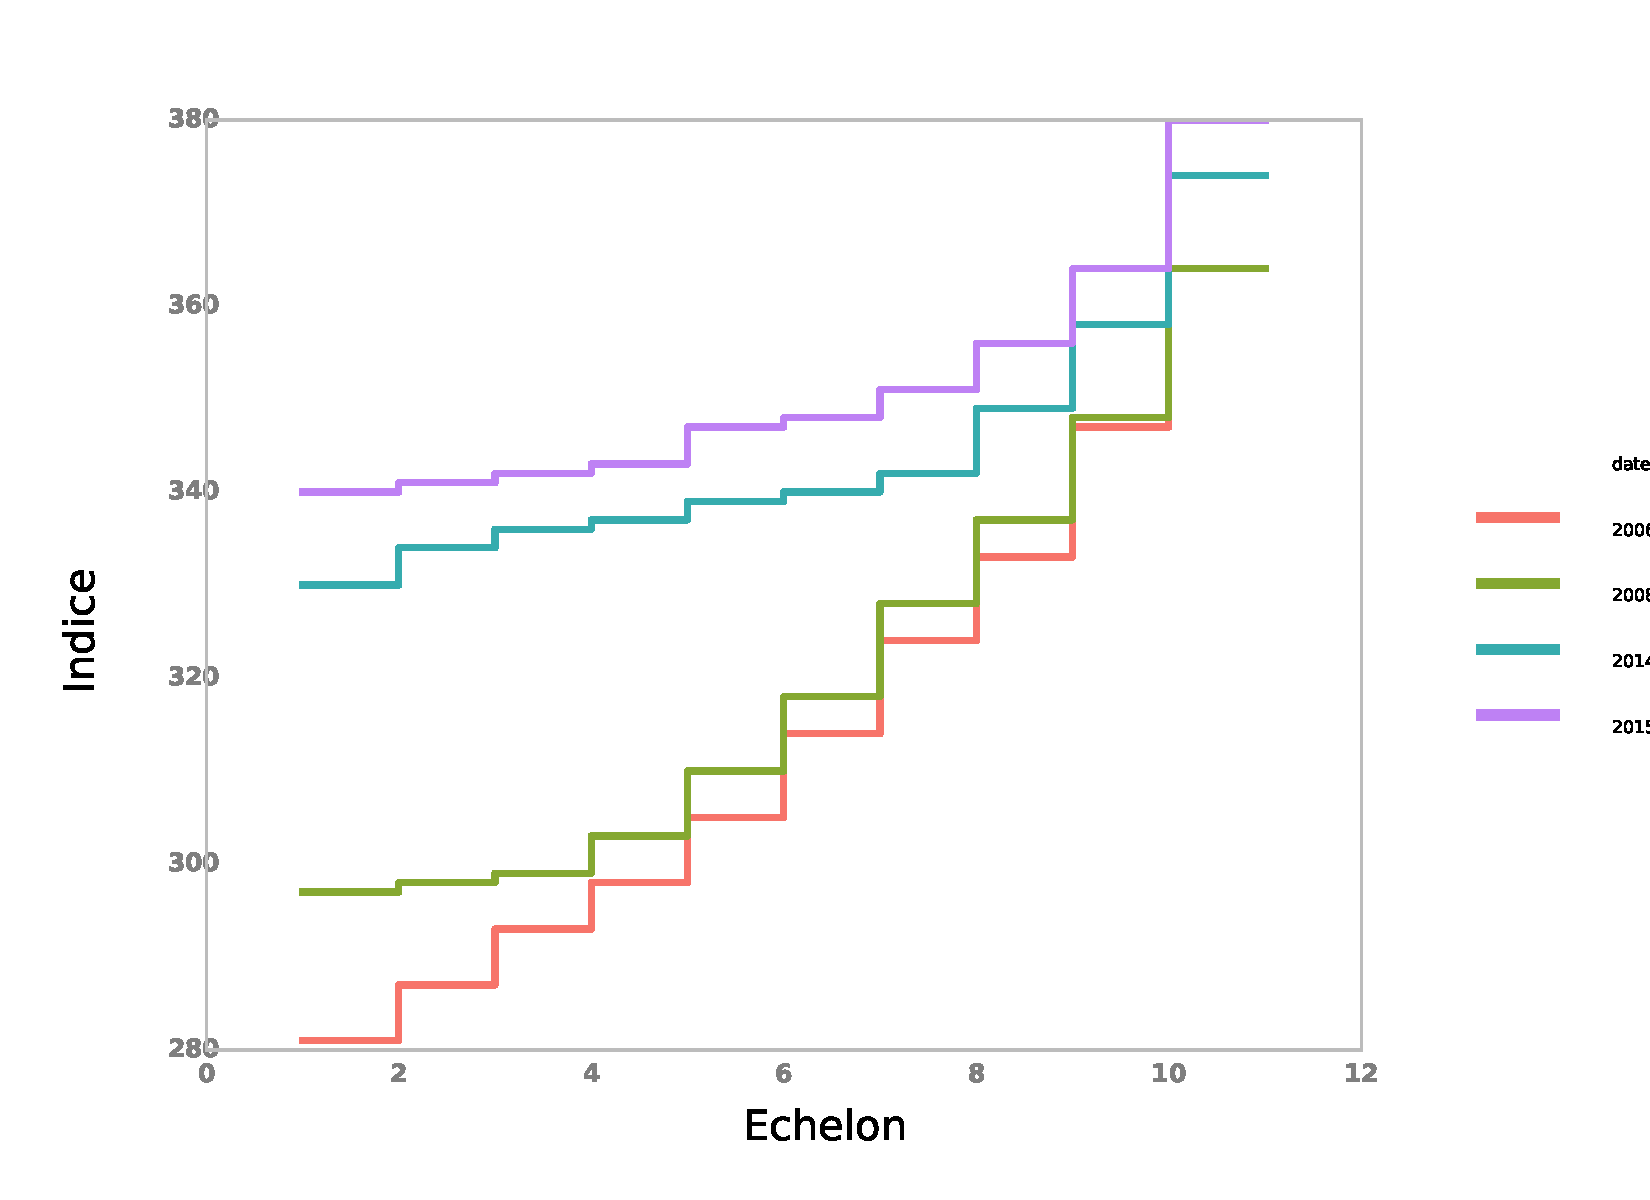
\includegraphics[width=1\linewidth]{0_grille_by_neg.pdf} 
    \vspace{4ex}
  \end{subfigure}%% 
  \begin{subfigure}[b]{0.55\linewidth}
        \caption{Grade 794} 
    \label{echelon_by_neg_1} 
    \centering
    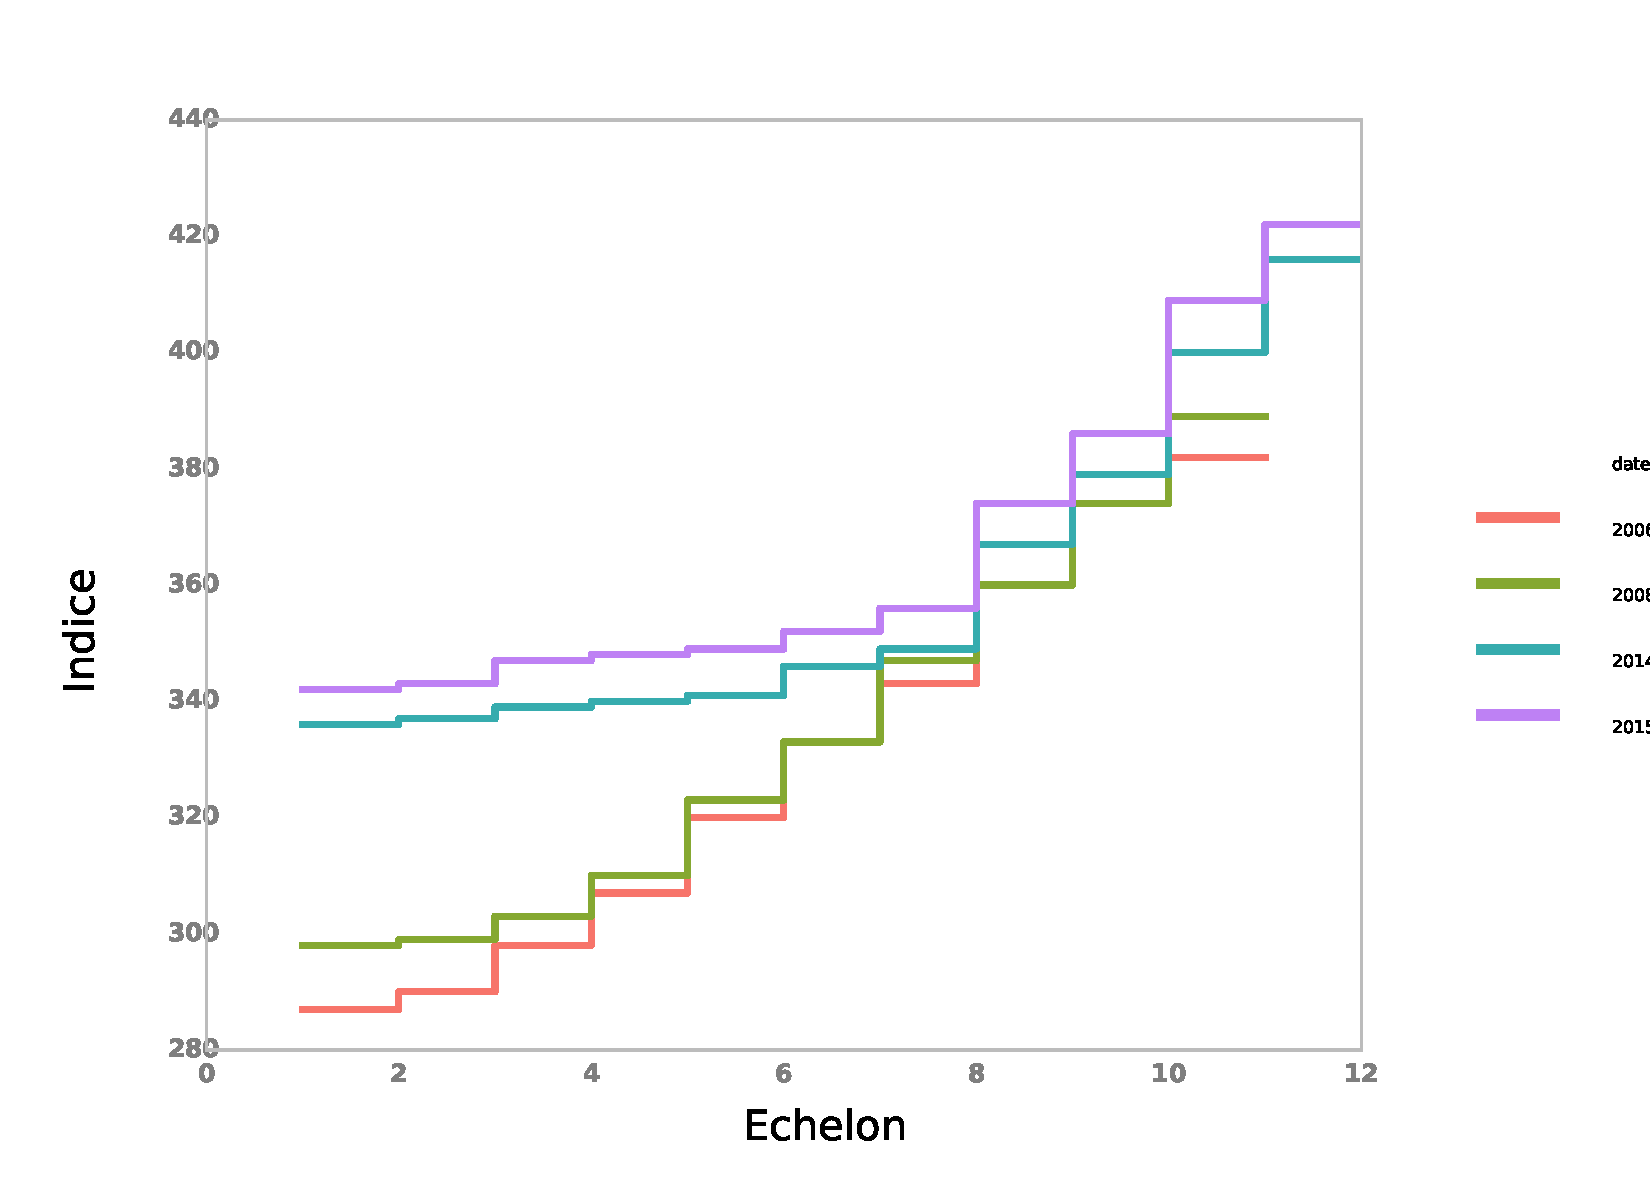
\includegraphics[width=1\linewidth]{1_grille_by_neg.pdf} 
    \vspace{4ex}
  \end{subfigure} 
  \begin{subfigure}[b]{0.55\linewidth}
        \caption{Grade 795} 
    \label{echelon_by_neg_2} 
    \centering
    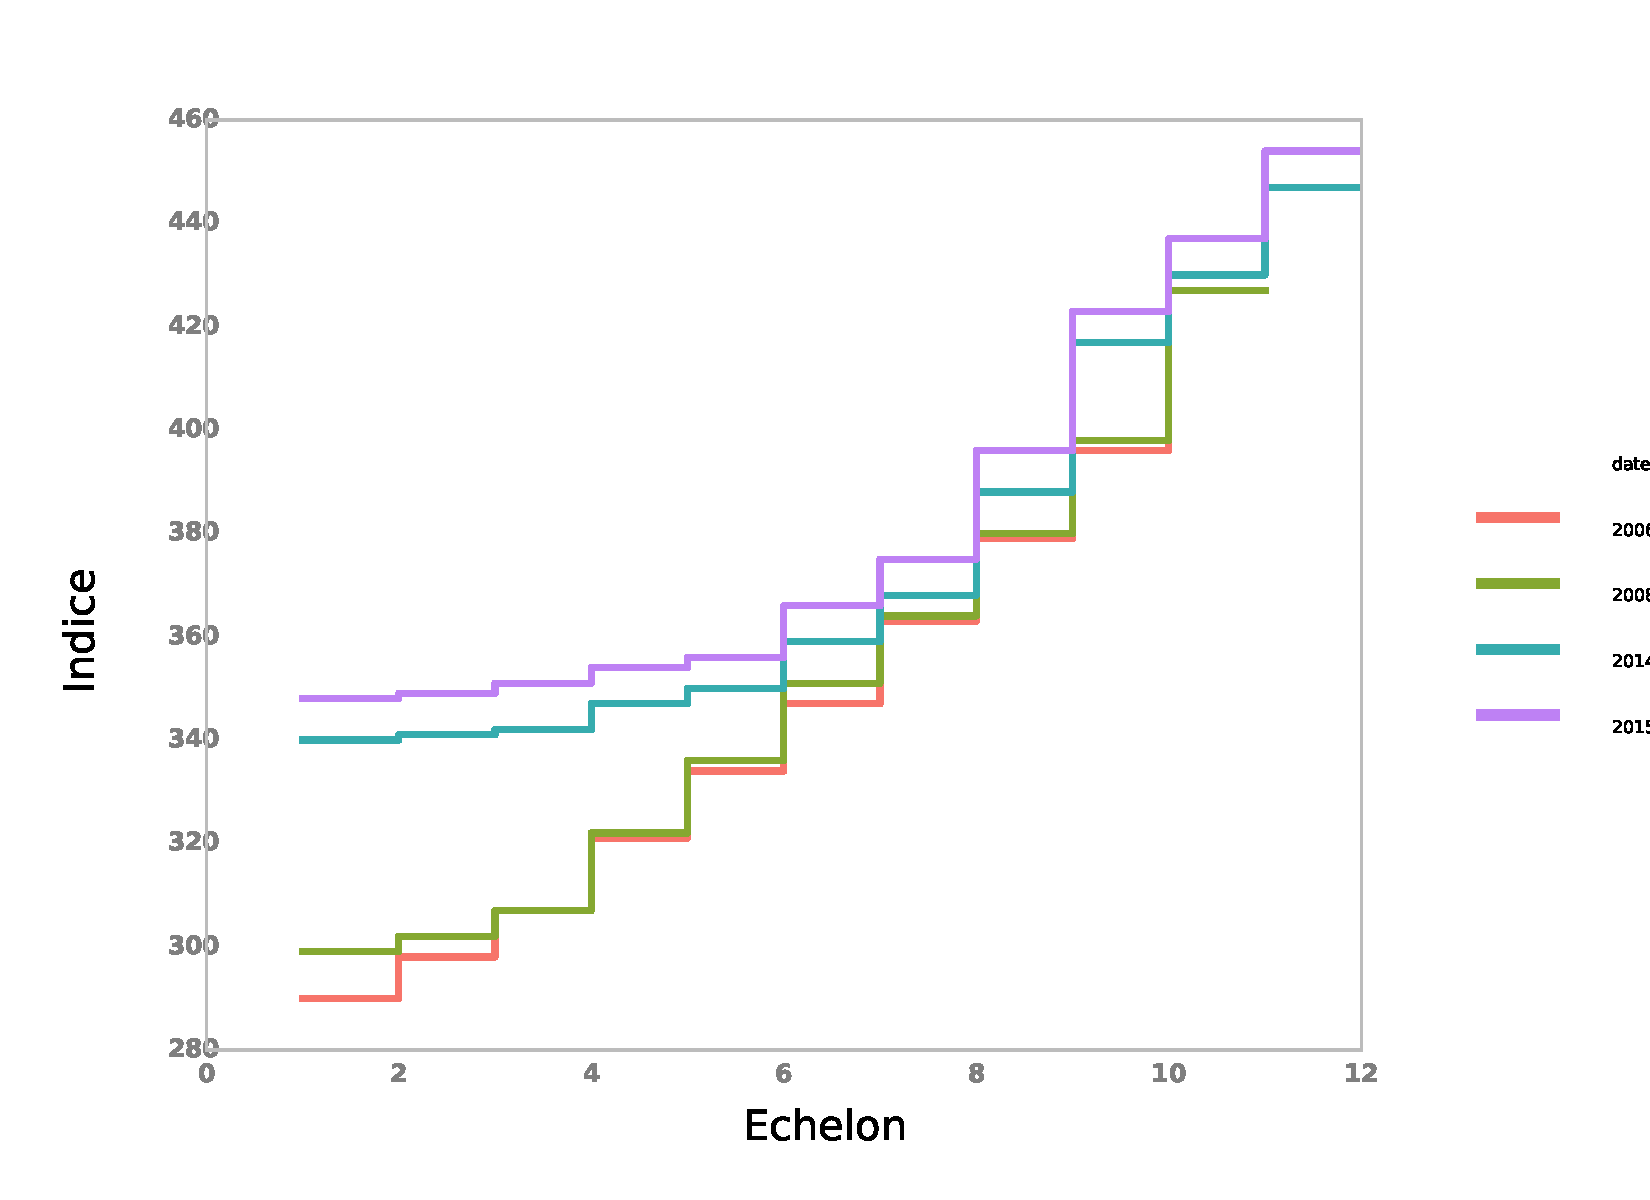
\includegraphics[width=1\linewidth]{2_grille_by_neg.pdf} 
  \end{subfigure}%%
  \begin{subfigure}[b]{0.55\linewidth}
        \caption{Grade 796} 
    \label{echelon_by_neg_3} 
    \centering
    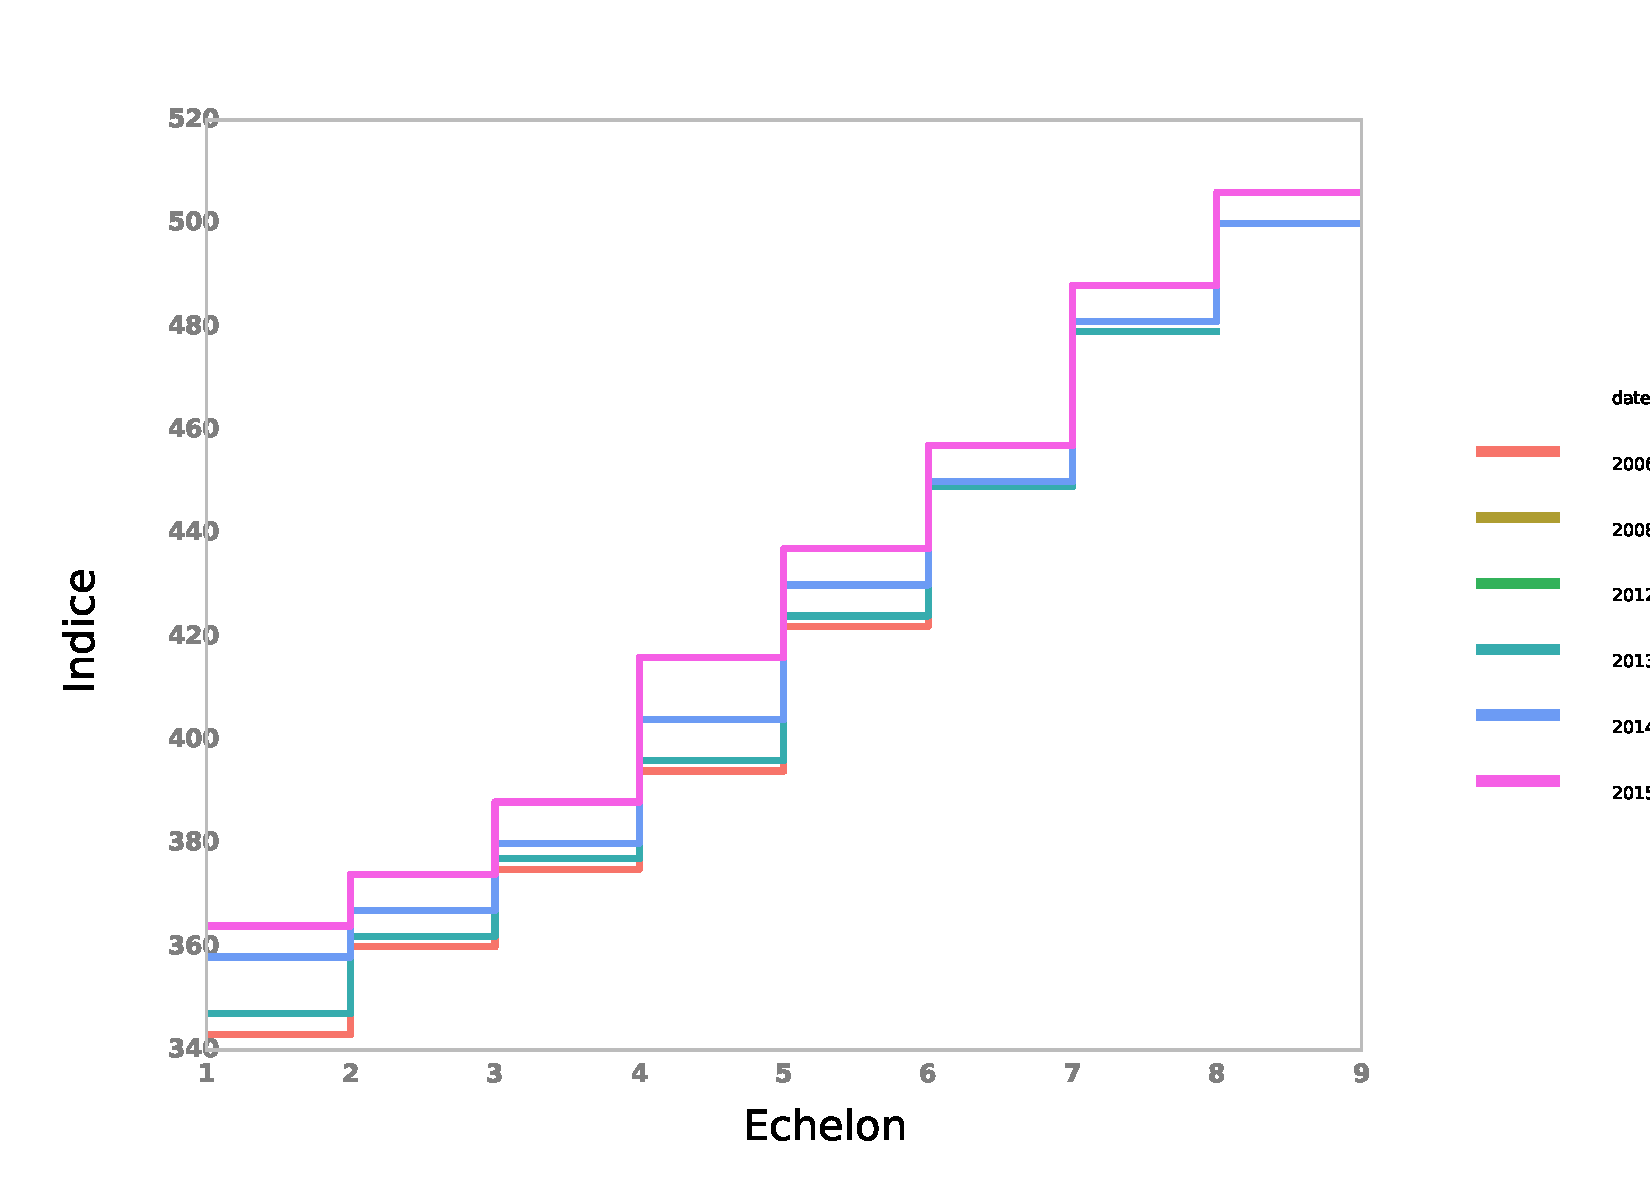
\includegraphics[width=1\linewidth]{3_grille_by_neg.pdf} 
  \end{subfigure} 
\end{figure}




\begin{figure}[ht] 
  \caption{Évolution des grilles: niveau relatif des grades}
  \label{echelon_by_date} 
  \begin{subfigure}[b]{0.55\linewidth}
      \caption{Année 2006} 
    \label{echelon_by_neg_0} 
    \centering
    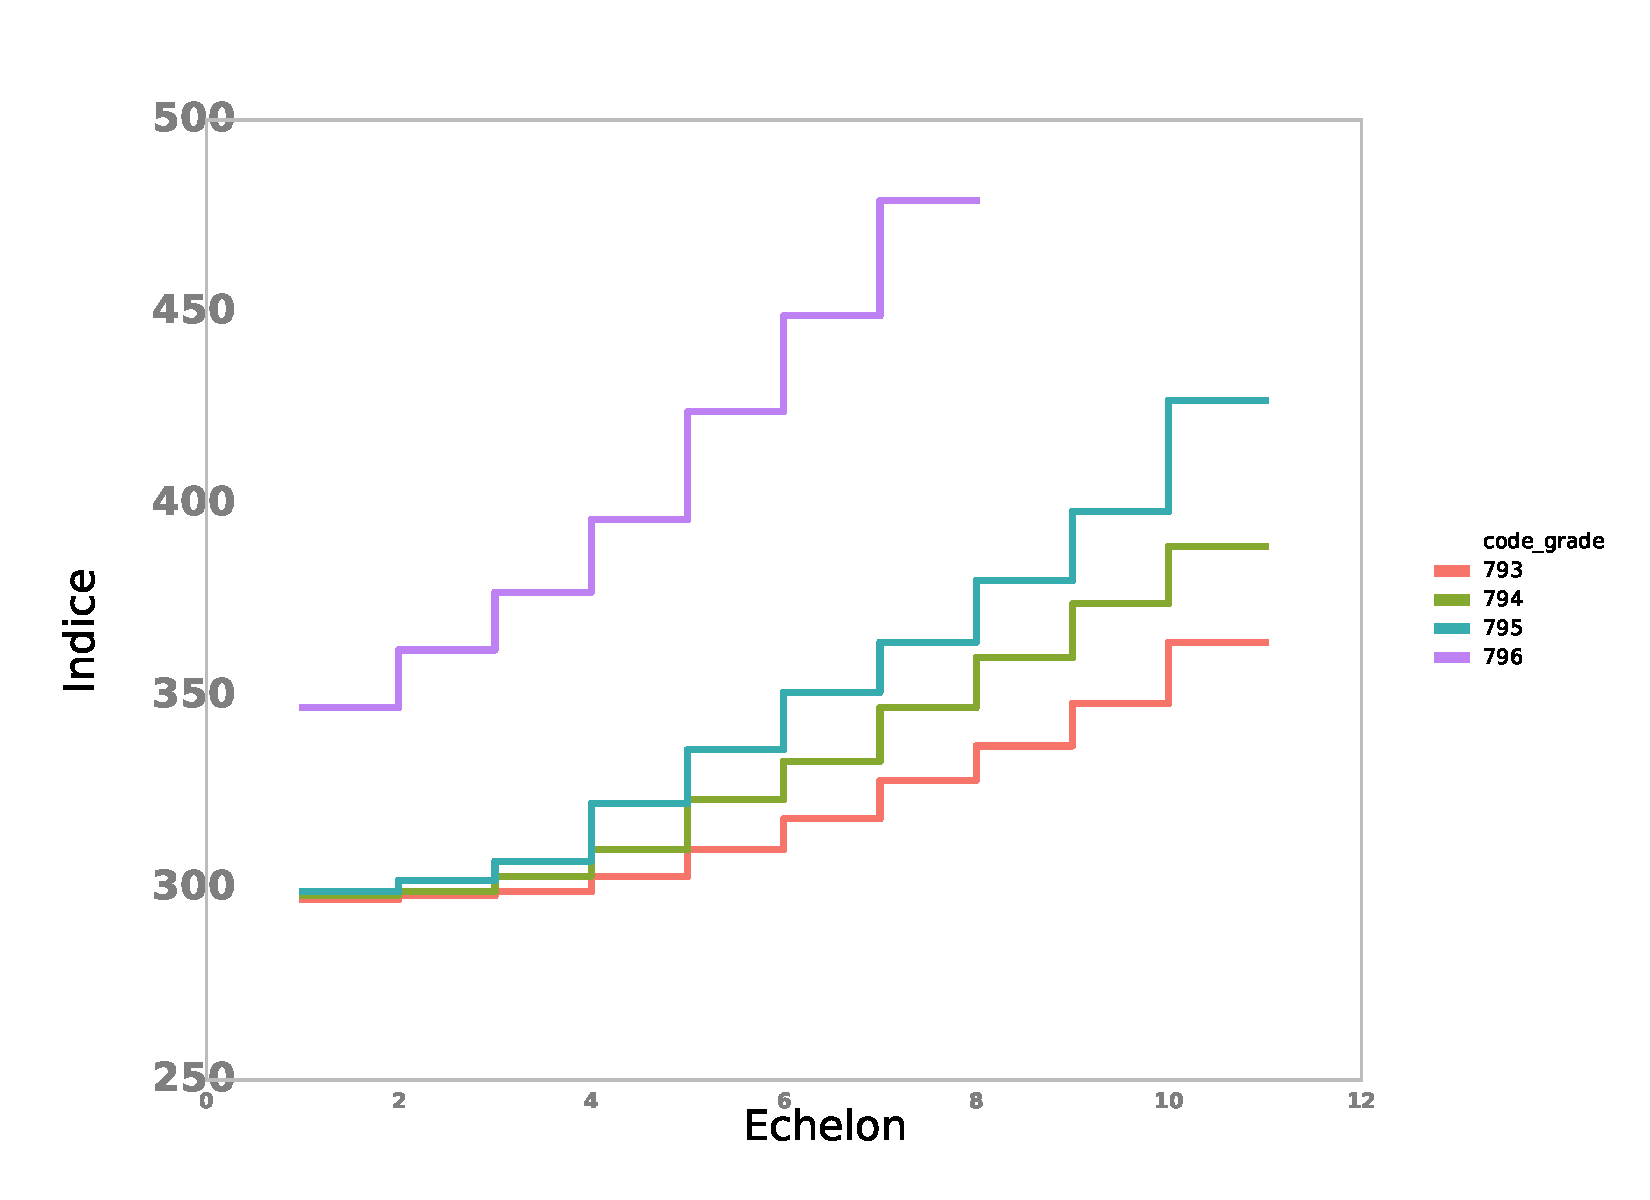
\includegraphics[width=1\linewidth]{0_grille_by_date.pdf} 
    \vspace{4ex}
  \end{subfigure}%% 
  \begin{subfigure}[b]{0.55\linewidth}
      \caption{Année 2008} 
    \label{echelon_by_neg_1} 
    \centering
    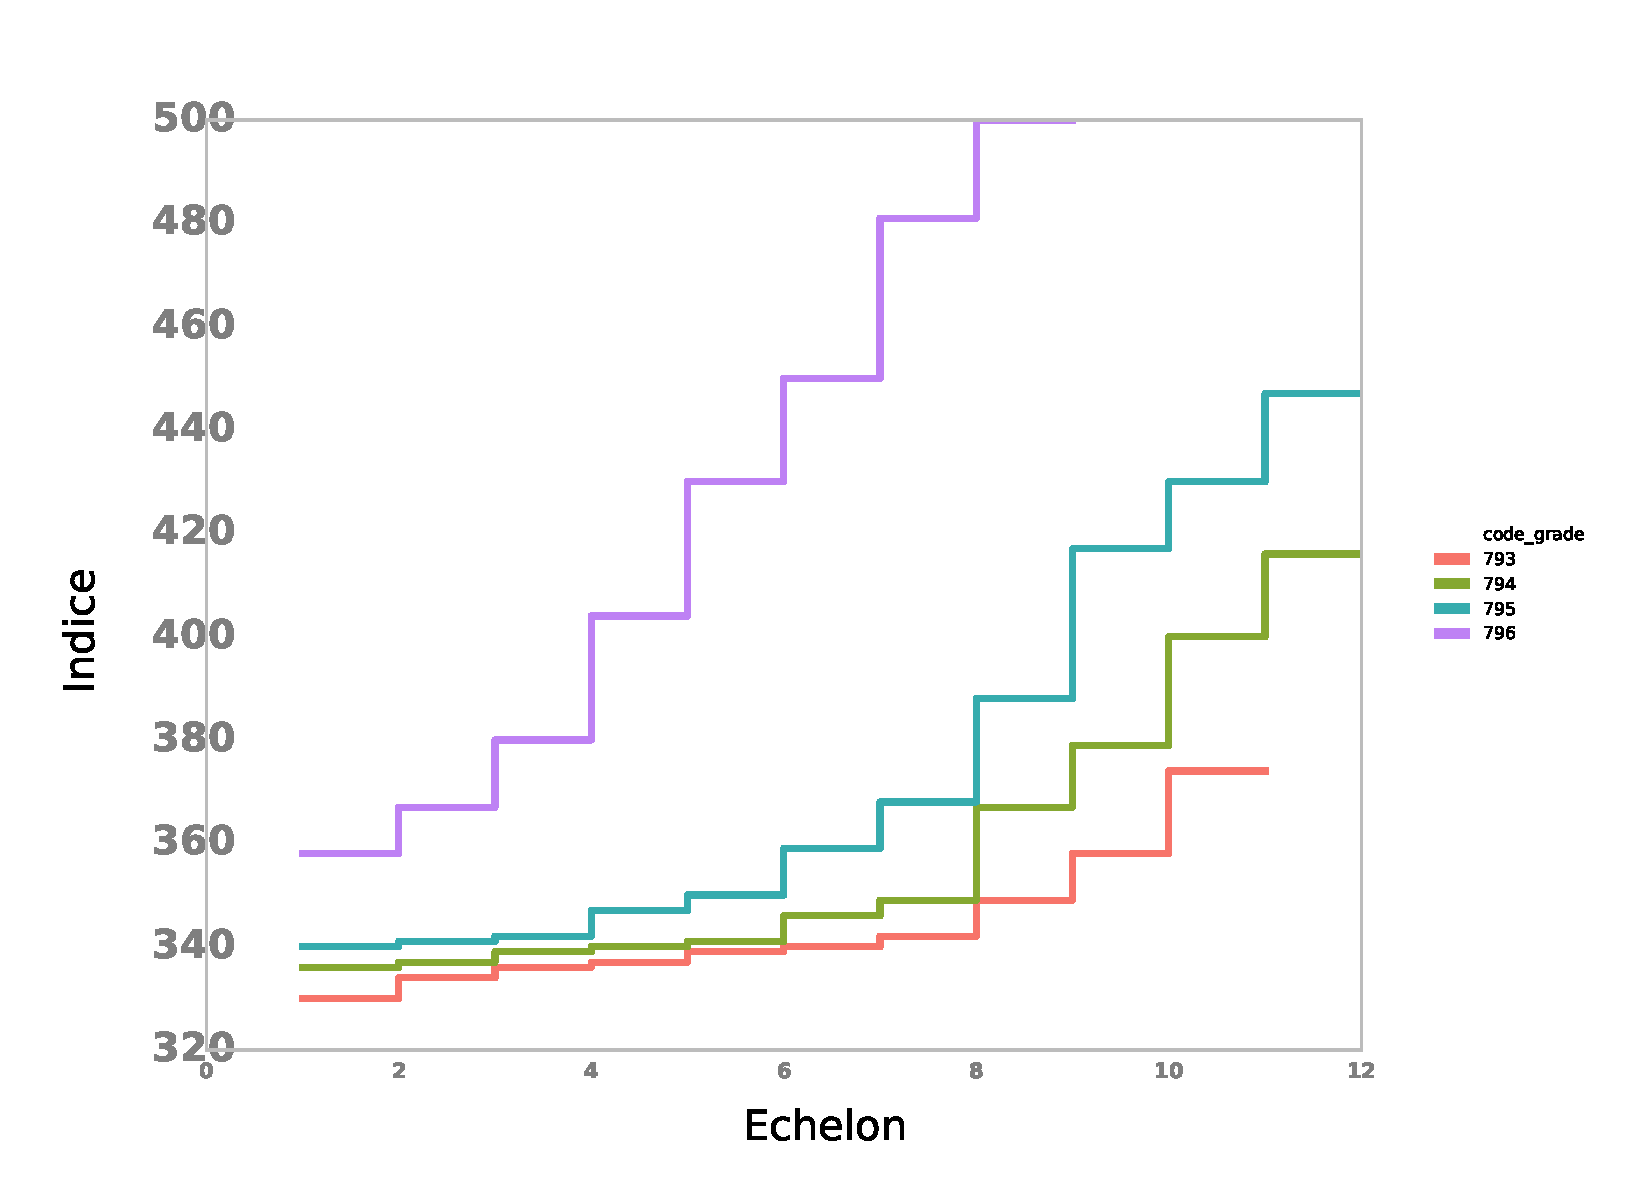
\includegraphics[width=1\linewidth]{1_grille_by_date.pdf} 
    \vspace{4ex}
  \end{subfigure} 
  \begin{subfigure}[b]{0.55\linewidth}
      \caption{Année 2014} 
    \label{echelon_by_neg_2} 
    \centering
    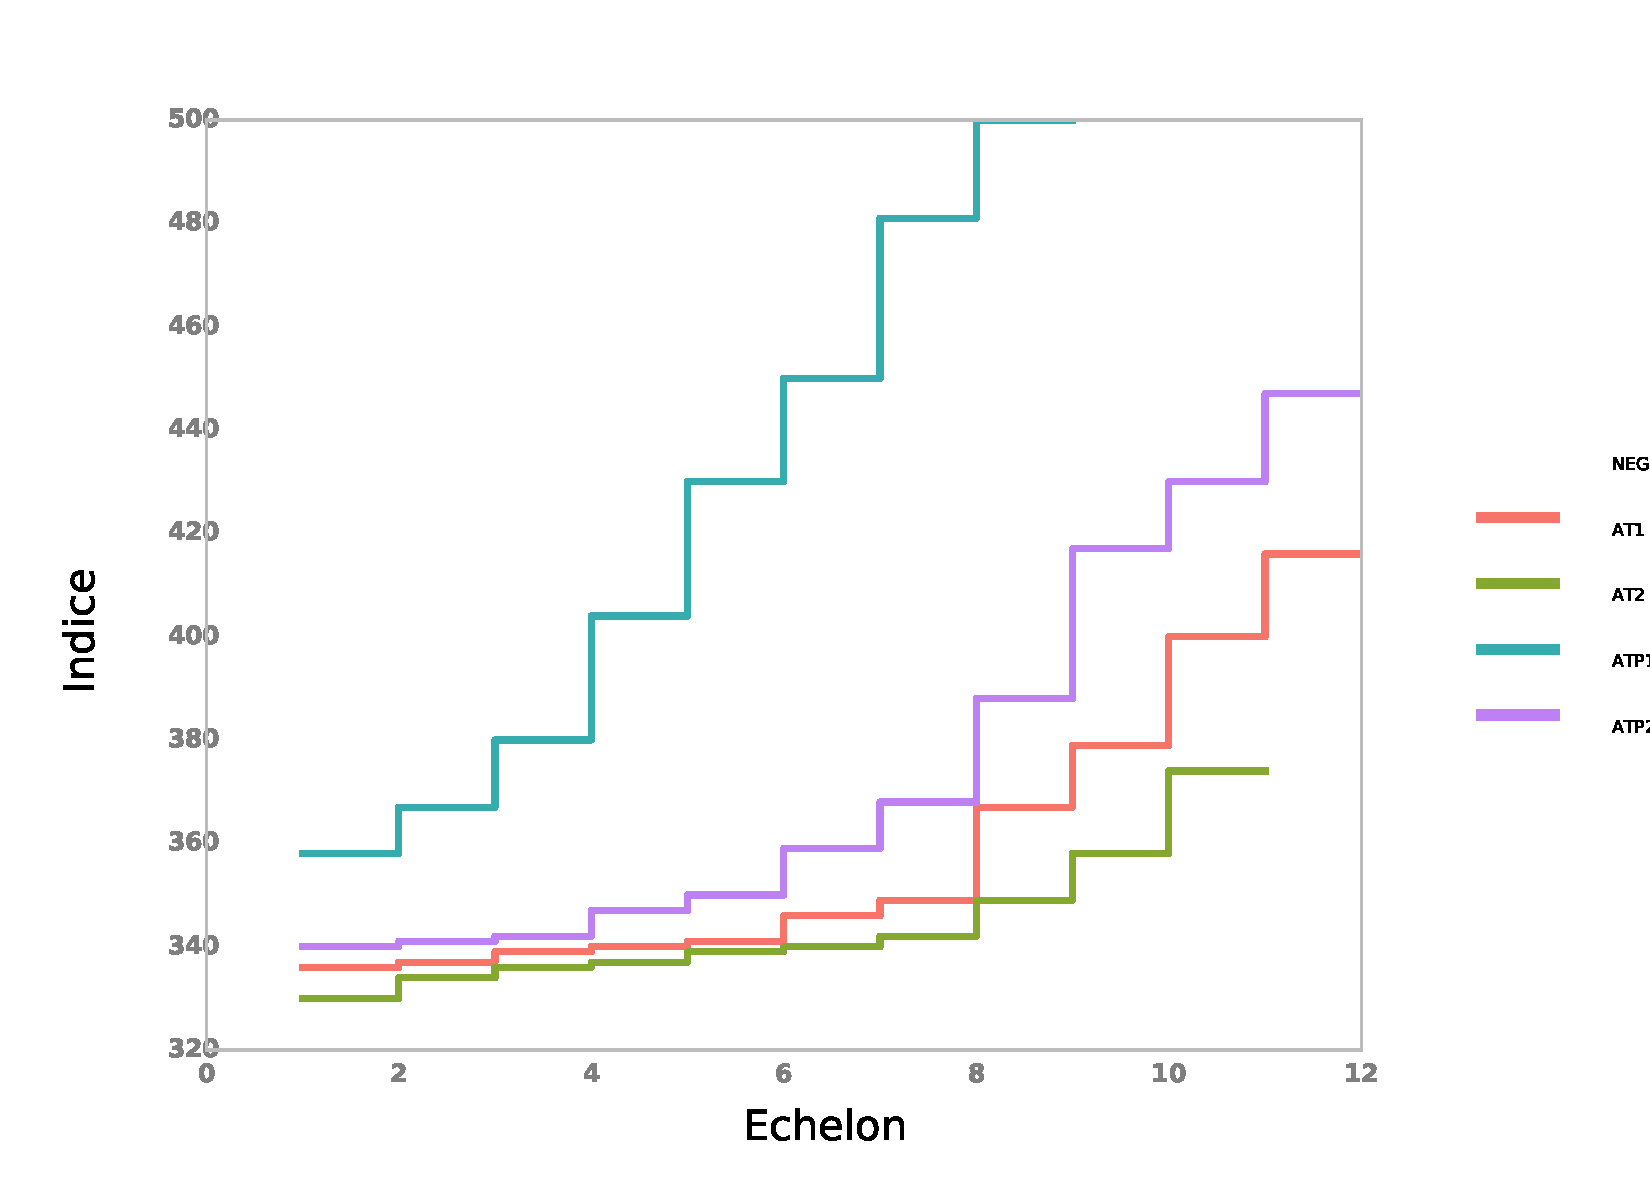
\includegraphics[width=1\linewidth]{2_grille_by_date.pdf} 
  \end{subfigure}%%
  \begin{subfigure}[b]{0.55\linewidth}
      \caption{Année 2015} 
    \label{echelon_by_neg_3} 
    \centering
    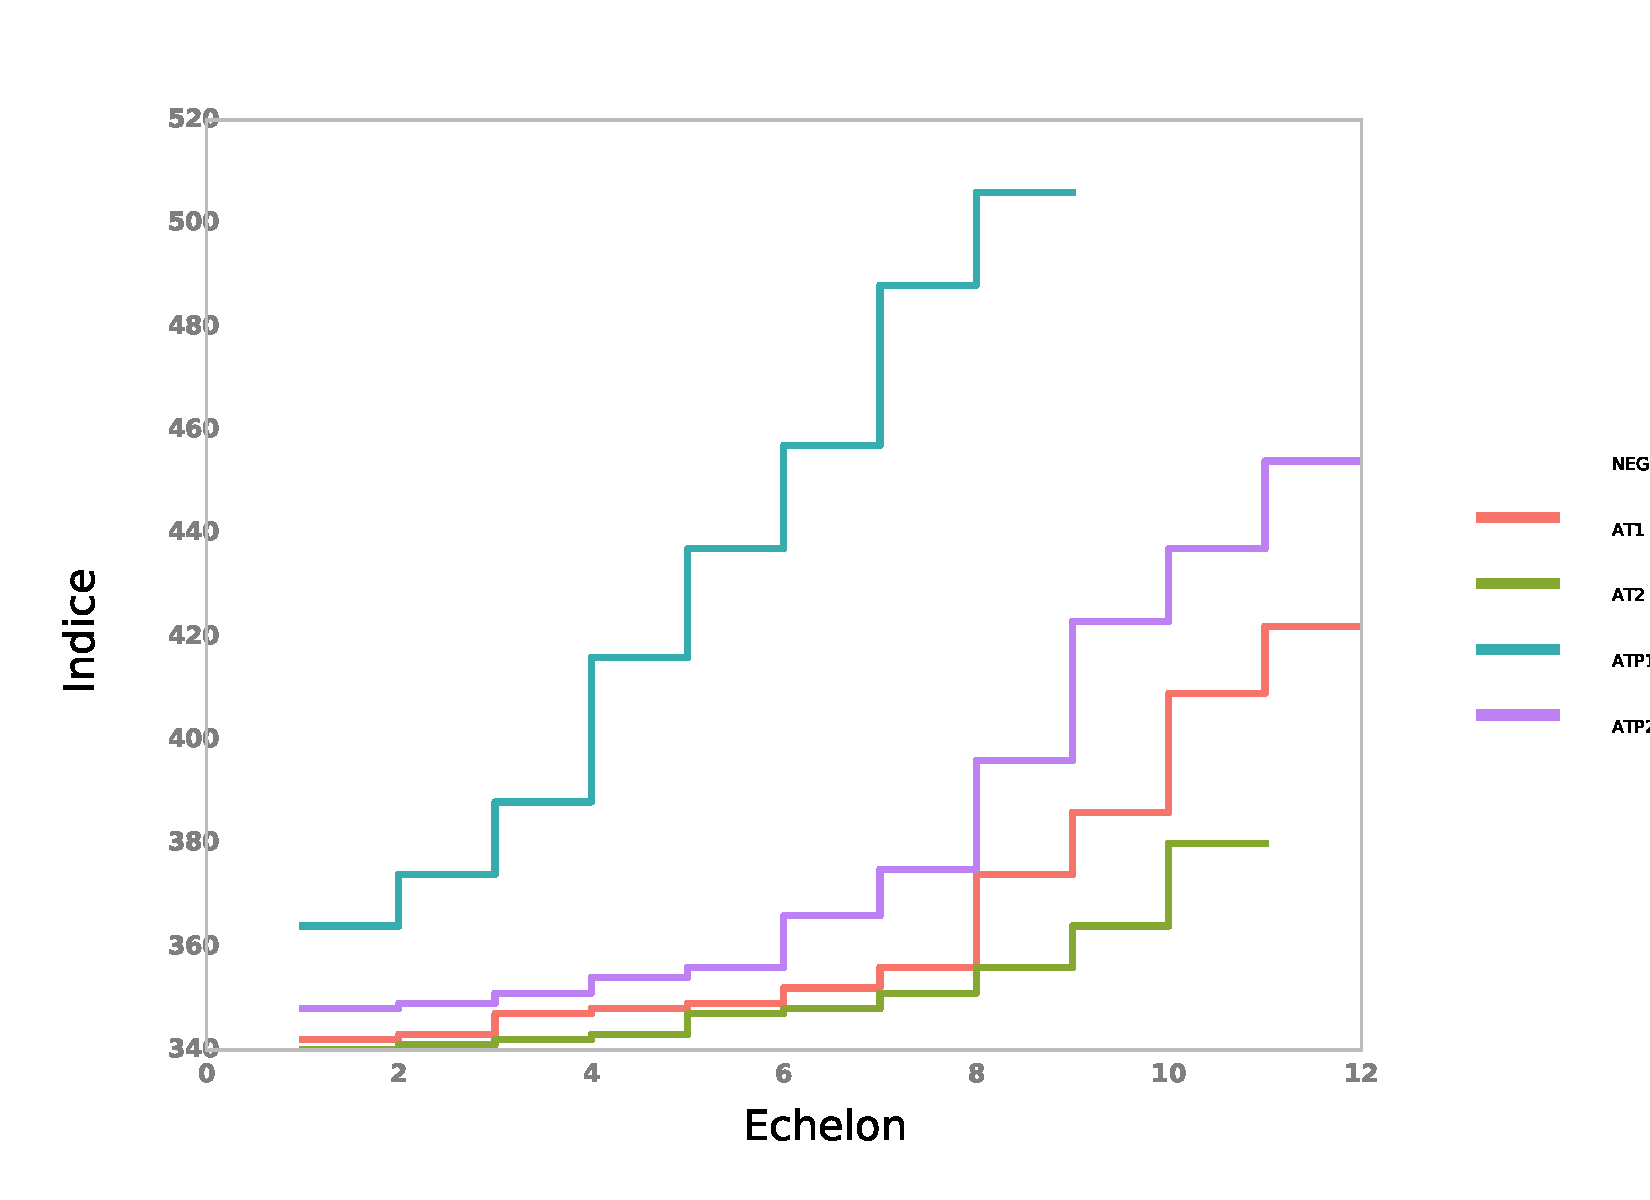
\includegraphics[width=1\linewidth]{3_grille_by_date.pdf} 
  \end{subfigure} 
\end{figure}




\clearpage





% Section II: Travail sur les données
\section{Point sur les données} \label{data}


\subsection{Sélection de l'échantillon}

Nous nous concentrons sur les individus, nés entre 1960 et 1999, et ayant passé au moins une année dans l'un des grades du corps. Nous supprimons les individus apparaissant deux fois (environ 250). Nous obtenus un échantillon initial d'environ 300,000 individus. 

L'étude des transitions entre grades et échelon nécessite de pouvoir identifier clairement les moments où le grade et l'échelon changent. La difficulté est alors la suivante: une information manquante pour l'une des variables clés rend difficile l'analyse de la séquence globale pour l'individu, car nous ne pouvons différencier une information manquante d'un changement dans la carrière. Le choix est pour l'instant fait de se concentrer sur une population restrictive, en ne gardant que les individus pour lesquels nous pouvons reconstituer la carrière de manière précise. 

Nous appliquons donc les filtres suivants à la base initiale. L'impact sur la taille de l'échantillon de ces filtres successifs est présenté à la table \ref{filters}. La règle appliquée est la suivante: dès que les conditions sont remplies pour au moins une observation dans la carrière de l'individu entre 2007 et 2015, nous retirons l'ensemble des observations pour l'individu en question. 
\begin{enumerate}[leftmargin=1cm ,parsep=0cm,itemsep=0cm,topsep=0cm] 
\item[F1] Garder uniquement les individus pour lesquels le libemploi n'est pas manquant quand l'indice ou le statut ne sont pas nuls. Nous perdons alors 15\% des individus, ce qui est relativement important par rapport à ce qui était attendu. 
\item[F2] Garder uniquement individus pour lesquels tous les grades sont renseignés, quand la variable libemploi n'est pas nulle. Cela implique de supprimer tous les individus pour lesquels les procédures d'imputation des libellés n'ont pas permis d'attribuer un grade neg pour chaque libemploi. Nous perdons ainsi 35\% des individus, ce qui était attendu. 
\item[F3] Garder uniquement les individus pour lesquels l'échelon est renseigné pour les années dans le corps. Ce filtre a un effet fort et inattendu, puisque l'on perd encore 12\% des individus. Par ailleurs cet effet est très hétérogène en fonction des grades. A cette étape les échelons manquant représentent environ 15\% des observations pour le grade AT2, contre 90\% pour le grade 795.
\end{enumerate}

La déperdition en étape F2 et F3 semble plus importante que ce que suggérait les statistiques descriptives pour les années les plus récentes. Cela suggère, comme précédemment soulignée\footnote{cf. mail Isabelle:  \\
\scriptsize
\begin{tabular}{lcccccccccccccc}
Année &2003&	2004 &	2005&	2006&	2007&	2008	&2010	&2011	&2012	&2013	&2014	&2015 \\
\% Neg renseigné & 15,4\%&	15,8 \% &	17,05	& 37,2 \%	&51,4 &	53,4 \% &	57,7 \%&	70,2 \%&	71,0 \% & 	71,4 \%	&71,5 \%&	71,6 \% \\
\% Ech renseigné &  3,9 \%	& 4,2 \%&	4,4 \%	&10,2 \% 	&25 \%	&24 \%	&33,5 \% &	54 \%&	56,3 \%&	58,2 \%	&58,5 \%	&58,9 \% \\
\end{tabular}
}, que la qualité de l'information de dégrade au cours du temps. 


\begin{table}[h!]
\centering
\caption{Impact des filtres successifs sur la taille de l'échantillon} 
\label{filters_AT}
\begin{tabular}{lcc}
\toprule
% latex table generated in R 3.1.0 by xtable 1.7-4 package
% Tue Mar 21 16:28:59 2017
 & Nb d'individus & \% echantillon initial \\ 
  \hline
Echantillon initial & 304367 & 100 \\ 
   \hline
F1: Libemploi manquant quand statut non vide & 265572 & 87 \\ 
  F2: Neg manquant quand libemploi renseigne & 145560 & 48 \\ 
  F3: Echelon manquant quand neg dans le corps & 108825 & 36 \\ 
   \hline
F3bis: Baisse d'echelon & 106890 & 35 \\ 
  F3ter: Saut d'echelon & 105032 & 35 \\ 
  
\bottomrule
\end{tabular}
\end{table}



\subsection{Qualité de l'information avant 2011}

Outre la question de l'alimentation des CIR, la dégradation de l'information au cours du temps peut s'expliquer par les différences dans le mode d'imputation du grade NEG avant et après 2011. En effet, après 2011 le grade est imputé sur la base du code NETNEH quand il est disponible, et avant l'imputation se fait sur la seule base du matching à partir des libellés saisis à la main. 

Une première illustration de la dégradation de l'information au cours du temps est présenté à la table \ref{quality1}. A partir d'une base pour laquelle seuls le filtre F1 (libemploi manquant), nous présentons l'évolution au cours du temps du taux de valeurs manquantes pour le grade et pour l'échelon. 
Nous re-constatons bien sur nous sous-population un taux de remplissage du grade qui chute avant 2011 (30\% de valeurs manquantes contre 12\% pour les années plus récentes). De manière encore plus marquée, nous observons une chute du taux de remplissage des échelons avant 2011. La proportion de valeurs manquantes est multipliée par trois avant 2011. Ce taux est par ailleurs variable d'une année à l'autre (43\% en 2007, 63\% en 2008) et d'un grade à l'autre (de 15\% à 100\% entre AT2 et 796). 

Ces chiffres doivent au préalables être confirmés et recoupés avec les analyses cotés CDC\footnote{En particulier pour le grade 796}, mais peuvent s'expliquer par au moins deux raisons: 
\begin{enumerate}
\item Un problème lié aux changements de grille (au niveau des collectivité ou de l'imputation), car les années marquées par des changements de grilles importants (2008, 2014) semblent particulièrement touchées). 
\item Un problème lié à une mauvaise imputation du grade sur la base des libellés remplis à la main à partir du matching. 
\end{enumerate}

Notons que l'on observe le même type de résultat pour le grade des adjoints administratifs (en particulier pour le dernier grade du corps), ce qui suggère que le problème n'est pas spécifique à la population sélectionnée.

Dans la suite du document, nous faisons le choix de ne pas étudier les échelons avant 2011, dans l'attente de pouvoir expliquer le nombre important de valeurs manquantes avant cette date. 



\begin{table}[h!]
\centering
\caption{Proportion de valeurs manquantes par années et par grade} 
\label{quality1}
\begin{tabular}{lccccccc}
\toprule
 & \%  lib NA & \% neg NA  & \% ech NA & \% ech NA   & \% ech NA   & \% ech NA  & \% ech NA  \\ 
&(statut rempli) & (lib rempli) & (neg rempli) & AT2 & 794 & 795 & 796 \\
\midrule 
% latex table generated in R 3.1.0 by xtable 1.7-4 package
% Tue Mar 21 16:54:53 2017
 & \% libemploi NA (statut OK) & \% c_neg NA (libemploi OK)  & \% ech NA & \% ech NA 793 & \% ech NA 794 & \% ech NA 795 & \% ech NA 796 \\ 
  \hline
2007 & 0.13 & 0.32 & 0.43 & 0.21 & 0.65 & 0.39 & 0.94 \\ 
  2008 & 0.08 & 0.31 & 0.63 & 0.59 & 0.57 & 0.64 & 0.99 \\ 
  2009 & 0.06 & 0.30 & 0.34 & 0.18 & 0.36 & 0.31 & 0.99 \\ 
  2010 & 0.04 & 0.29 & 0.32 & 0.15 & 0.34 & 0.38 & 1.00 \\ 
  2011 & 0.01 & 0.12 & 0.09 & 0.06 & 0.06 & 0.13 & 0.94 \\ 
  2012 & 0.01 & 0.12 & 0.09 & 0.06 & 0.06 & 0.13 & 0.99 \\ 
  2013 & 0.01 & 0.12 & 0.08 & 0.07 & 0.08 & 0.13 & 0.05 \\ 
  2014 & 0.01 & 0.13 & 0.16 & 0.15 & 0.17 & 0.22 & 0.14 \\ 
  2015 & 0.00 & 0.13 & 0.09 & 0.08 & 0.09 & 0.14 & 0.05 \\ 
   \hline
 
\bottomrule
\end{tabular}
\end{table}


La table \ref{quality2} permet de comprendre les conséquences de cette rupture statistique sur l'analyse des trajectoire présente l'évolution de la proportion de changement d'une année à l'autre, proportion qui est décomposée en fonction des différents types de changements possible (de grade manquant à grade renseignée, de grade renseigné à grade manquant, et de grade à grade). 
Nous constatons à l'année 2011 une forte augmentation de la probabilité de changement de grade. Cette augmentation est liée à deux facteurs: 
\begin{enumerate}
\item Une hausse des transitions de grade manquant vers grade renseigné, qui découle du meilleur remplissage de la variable neg à partir de 2011, qui conduit à l'apparition de nouveaux individus à partir de 2011.  
\item Une mauvaise imputation du grade avant 2011, qui conduit à une hausse fictive des changements de grade à grade qui traduisent simplement la correction induite par l'imputation du grade neg sur la base du NETNEH. 
\end{enumerate}
 

\begin{table}[h!]
\centering
\caption{Proportion de changements de grade par année} 
\label{quality2}
\begin{tabular}{lcccccccc}
\toprule
Année & 2008 & 2009 & 2010 & 2011 & 2012 & 2013 & 2014 & 2015 \\[0.2em]
\midrule
Filtre F1 &&&&&& \\ \midrule
% latex table generated in R 3.1.0 by xtable 1.7-4 package
% Fri Mar 24 13:11:05 2017
 \% Changement de grade & 0.15 & 0.16 & 0.15 & 0.45 & 0.16 & 0.15 & 0.15 & 0.17 \\ 
   \hline
\%  de NA a grade & 0.07 & 0.07 & 0.07 & 0.22 & 0.07 & 0.05 & 0.05 & 0.04 \\ 
  \% de grade a NA & 0.03 & 0.03 & 0.03 & 0.06 & 0.03 & 0.02 & 0.03 & 0.04 \\ 
  \%  de grade a grade & 0.04 & 0.05 & 0.05 & 0.17 & 0.06 & 0.07 & 0.07 & 0.09 \\ 
   
&&&&&& \\ 
Filtre F2 &&&&&& \\ \midrule
% latex table generated in R 3.2.1 by xtable 1.8-2 package
% Sat Apr 01 16:21:55 2017
 \% Changement de grade & 0.11 & 0.11 & 0.12 & 0.30 & 0.13 & 0.15 & 0.15 & 0.17 \\ 
   \hline
\%  de NA a grade & 0.06 & 0.05 & 0.05 & 0.06 & 0.06 & 0.06 & 0.06 & 0.05 \\ 
  \% de grade a NA & 0.00 & 0.00 & 0.00 & 0.01 & 0.01 & 0.01 & 0.01 & 0.03 \\ 
  \%  de grade a grade & 0.05 & 0.07 & 0.07 & 0.23 & 0.06 & 0.08 & 0.08 & 0.10 \\ 
     
&&&&&& \\
Filtre F3 &&&&&& \\ \midrule
% latex table generated in R 3.2.1 by xtable 1.8-2 package
% Sat Apr 01 16:21:55 2017
 \% Changement de grade & 0.10 & 0.10 & 0.11 & 0.26 & 0.14 & 0.15 & 0.16 & 0.18 \\ 
   \hline
\%  de NA a grade & 0.05 & 0.05 & 0.05 & 0.08 & 0.07 & 0.08 & 0.08 & 0.06 \\ 
  \% de grade a NA & 0.00 & 0.00 & 0.00 & 0.01 & 0.01 & 0.01 & 0.01 & 0.03 \\ 
  \%  de grade a grade & 0.05 & 0.05 & 0.06 & 0.17 & 0.06 & 0.07 & 0.08 & 0.09 \\ 
     
\bottomrule
\end{tabular}
\begin{minipage}{12cm}
\footnotesize
\textsc{Population:} Population initiale avec application des filtres successifs.
\end{minipage}
\end{table}




\subsection{Censure des données}

Les données dont on dispose sont censurées, car nous observons les trajectoires uniquement entre 2007 (choix de profondeur) et 2015 (dernière année disponible). Quelque soit le processus que l'on considère (passage dans un corps, dans un grade, dans un échelon), celui-ci sera observé de manière potentiellement incomplète. Comme illustré sur le schéma de la figure  \ref{censure}, la censure peut être de différent type. Si l'ensemble de la séquence se déroule entre 2007 et 2015, nous n'avons pas de censure (cas 1). La censure peut ensuite être à gauche si le processus est débuté avant 2007 (cas 2) ou à droit s'il est s'achève après 2015 (cas 3). Il peut également y avoir censure des deux cotés (cas 4). 

Notons que le problème de censure est naturellement plus aigu pour les processus longs. Ce sera sans doute le cas pour la modélisation de la trajectoire dans le grade. Par exemple, si l'on prend la grille qui a cours en 2008, la durée minimale (resp. maximale) pour parcourir l'ensemble du grade est de 21 (resp. 30) ans. Si la plupart des individus ne parcourent pas l'ensemble d'un grade, nous risquons d'être confronté à ce problème, même si nous disposons de données propres de 2007 à 2015. 

Soulignons que la censure à gauche est plus problématique que la censure à droite. En cas de censure à droite, nous pouvons tout de même utiliser l'information disponible: l'individu est resté dans le grade donné jusqu'en 2015. Dans  le cas de la censure à gauche, nous devons obligatoirement imputer l'état initial, la durée déjà passée dans le grade avant 2007, ce qui ne peut se faire de manière simple. 

Notons enfin que nous ne sommes pas dans un cas de censure totale, puisqu'il est possible d'utiliser les informations sur les variables avant 2007 (libellés emploi, indice, date d'affiliation, etc). 


\begin{figure}[H] 
  \caption{Censure des données: illustration}
  \label{censure} 
    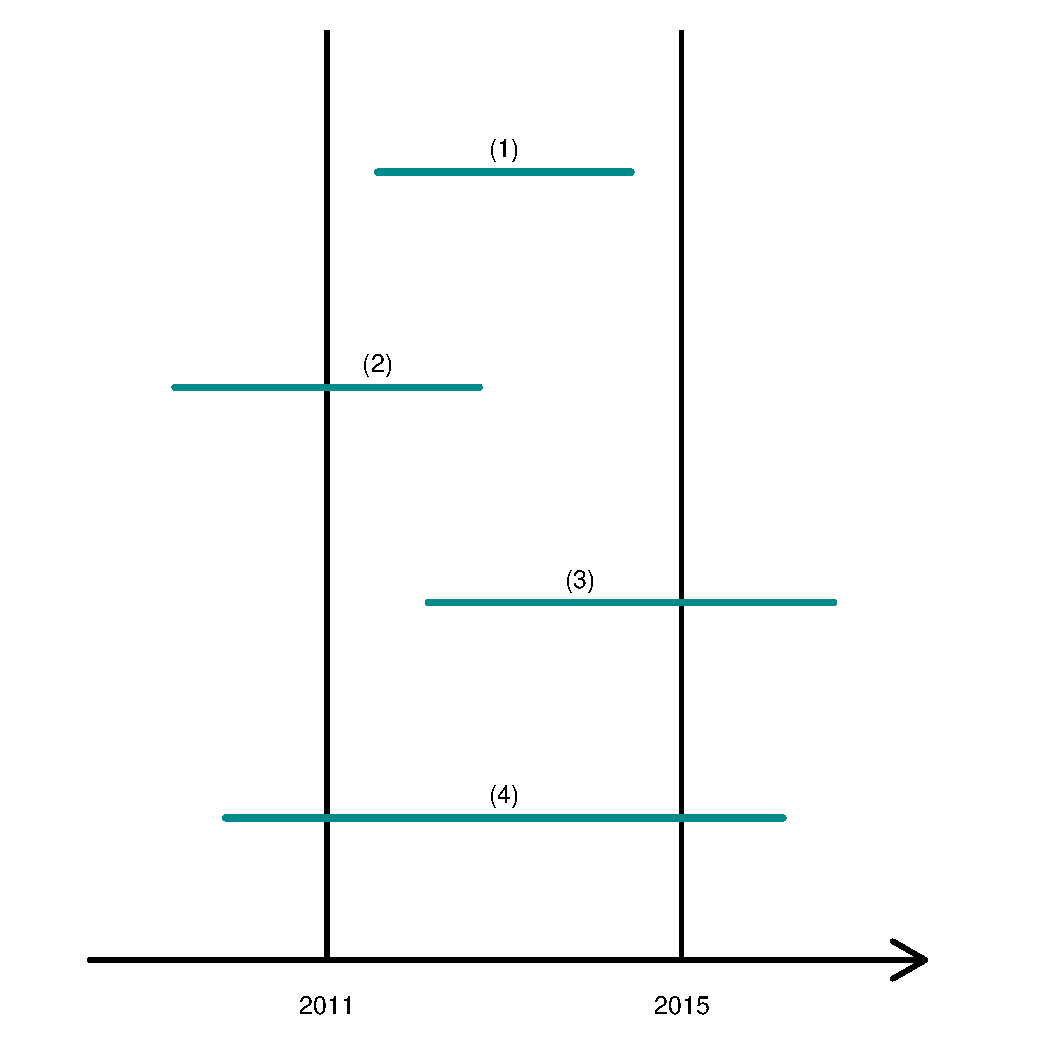
\includegraphics[scale = 0.5]{schema_censoring.pdf} 
\end{figure}



% Section III: Statistiques descriptives
\section{Analyse des trajectoires: statistiques descriptives}

Dans cette section nous présentons des statistiques descriptives permettant de décrire les trajectoires dans les grilles de la population considérée. 

\subsection{Trajectoires indiciaires}

Une première illustration des trajectoires de rémunération est proposée à la figure \ref{trajectories}. Elle présente l'évolution par année de l'indice pour une sous-population particulière, des individus dont l'année d'affiliation au régime est 2007, et qui passent ensuite l'ensemble de leur carrière dans le corps des adjoints techniques. Nous représentons en bleu les changements de grilles et en rouge les changements de grade entre deux années. 

De manière intéressante, nous observons des trajectoires en "escalier", qui traduisent l'évolution des grilles et des individus dans ces grilles. Les marches les plus importantes sont générées par des changements de grille ou des changements de grade. Même s'il s'agit d'une population aux trajectoires particulièrement simples, ces exemples soulignent la pertinence de l'approche par grilles. En effet, une simple équation de salaire ne saurait reproduire ce type d'évolution. 

A titre d'illustration, la figure \ref{trajectories_D} présent des exemples (représentatifs cette fois) de trajectoires salariales issues des projections du modèle Destinie de l'Insee. Conformément à ce qui est attendu, les équations de salaires usuellement mises en place conduisent à des profils d'évolution linéaires, peut-être  adaptés pour les salariés du privé, mais moins pour les carrières des fonctionnaires. 


\begin{figure}[H] 
\caption{Exemples de trajectoires indicaires}
\label{trajectories} 
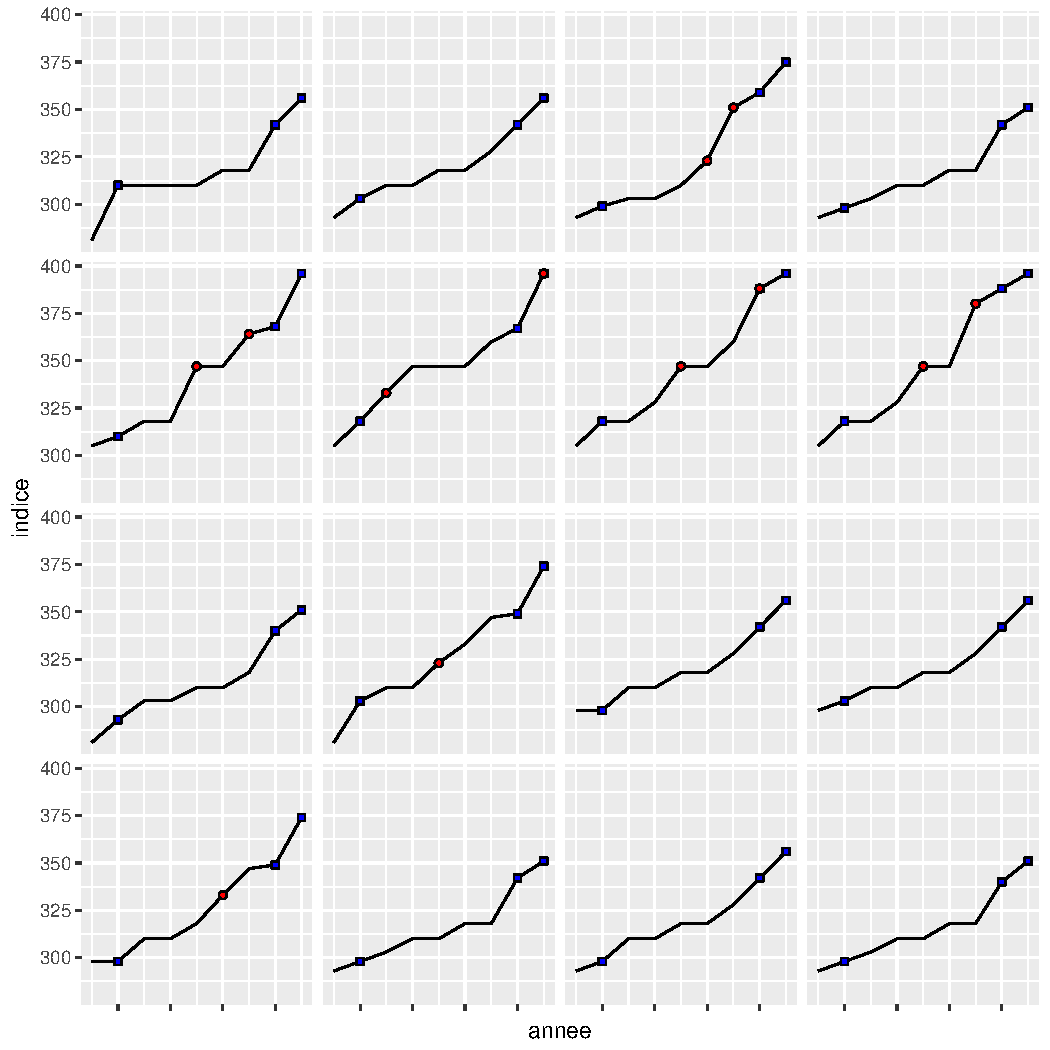
\includegraphics[width=1\linewidth]{trajectoires.pdf} 
\begin{minipage}{15cm}
\footnotesize
\textsc{Population:} Individus qui font leur entrée dans le régime en 2007 au grade 793, et qui connaissent toutes leur carrière dans le corps. \\
\textsc{Note:} Les carrés bleus correspondent à des années de changement de grille, les ronds rouges à des années de changement de grade. 
\end{minipage}
\end{figure}



\begin{figure}[H] 
\caption{Exemples de trajectoires salariales projetées dans Destinie}
\label{trajectories_D} 
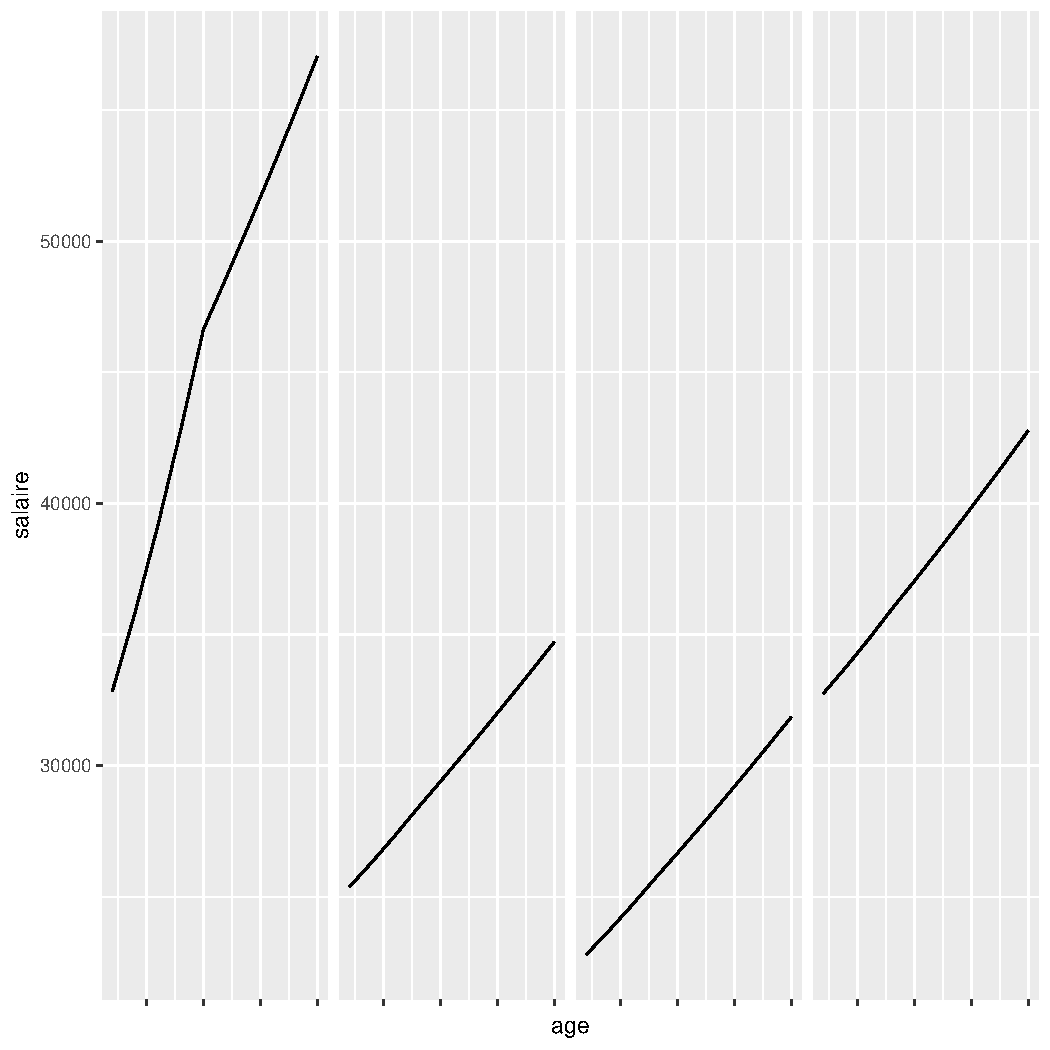
\includegraphics[width=1\linewidth, height = 0.5\linewidth]{trajectoires_D.pdf} 
\begin{minipage}{12cm}
\footnotesize
\textsc{Population:} Individus nés en 1990 avec des salaires > 0 entre 30 et 40 ans. \\
\textsc{Source:} Modèle Destinie de l'Insee
\end{minipage}
\end{figure}


\bigskip

\subsection{Grade de provenance et de destination}


Une question importante dans la modélisation des trajectoires est le niveau adéquat de modélisation. L'approche par corps adoptée ici se justifie-t-elle? Ou est-elle déjà trop large car les liens entre les différents grades du corps ne sont pas si importants, ou trop réduite car l'on néglige des dynamiques avec d'autres corps (de la filière, ou d'une autre filière). 

La définition du bon niveau d'analyse devrait pouvoir se déterminer directement à partir des données, par l'étude des réseaux générés par les différentes transitions. Dans l'attente de développer une telle analyse, nous décrivons simplement les transitions pour les grades étudiés. Nous présentons d'une part les grades de provenance (table \ref{entry}) et les grades de destinations (table \ref{exit}) pour les grades étudiés. 

Nous nous concentrons sur les transitions ayant lieu dans les années plus récentes, pour lesquelles l'information est la plus fiable. Nous n'appliquons par le filtre F3 sur les échelons car nous travaillons uniquement sur les grades. 

\bigskip

Pour ce qui est des grades de provenance, nous soulignons les points suivants: 
\begin{enumerate}[leftmargin=1cm ,parsep=0cm,itemsep=0cm,topsep=0cm] 
\item L'approche par corps semble bien justifiée: une très grande majorité des individus se trouvant dans un grade donné provient du grade immédiatement précédent dans le corps (sauf pour le premier grade 793, qui correspond aux premières affiliations).  
\item Nous observons des transitions a priori surprenantes voire impossibles d'un grade supérieur vers un grade inférieur.  
\end{enumerate}

\medskip

Pour ce qui est des grades de destination, nous soulignons les points suivants: 
\begin{enumerate}[leftmargin=1cm ,parsep=0cm,itemsep=0cm,topsep=0cm] 
\item Il y a également une forte détermination du corps dans les trajectoires, le corps suivant étant toujours la principale destination. 
\item Ce constat est moins vrai pour le premier grade du corps, pour lequel on observe plus de transition vers l'extérieur. Cela s'explique peut-etre par la structure pyramidale du corps: s'il y a moins de poste pour les grades supérieurs, tout le monde ne peut pas passer au grade supérieur ("up or out"). 
\item Parmi ces 24\% de départs depuis le grade 793 vers des autres grades, la principale destination est le grade d'adjoint administratif de deuxième classe (17\% du total des destinations). Cela suggère des liens potentiellement importants entre ces deux corps.
\end{enumerate}


\medskip

\begin{table}[h!]
\centering
\caption{Répartition des grades de provenance} 
\label{entry}
\begin{tabular}{lcccc}
\toprule
 & \multicolumn{4}{c}{Grade en n (changement en n)} \\
 & 793 & 794 & 795 & 796 \\ 
  \hline
% latex table generated in R 3.1.0 by xtable 1.7-4 package
% Fri Mar 24 13:12:53 2017
 NEG n-1 = 793 & 0.00 & 79.39 & 4.39 & 1.00 \\ 
  NEG n-1 = 794 & 2.30 & 0.00 & 82.05 & 0.84 \\ 
  NEG n-1 = 795 & 0.13 & 0.15 & 0.00 & 92.14 \\ 
  NEG n-1 = 796 & 0.01 & 0.15 & 0.00 & 0.00 \\ 
   \hline
NEG n-1 = autres & 5.87 & 2.18 & 2.46 & 1.17 \\ 
   \hfill dont le grade  & 791 & 791 & 792 & 14 \\ 
  \hfill  representant  & 4.36 & 0.89 & 0.83 & 0.67 \\ 
   \hfill dont le grade  & 807 & 792 & 791 & 162 \\ 
  \hfill  representant  & 0.34 & 0.80 & 0.79 & 0.33 \\ 
   \hline
NEG n-1 = manquant & 91.68 & 18.13 & 11.11 & 4.85 \\ 
  total & 100.00 & 100.00 & 100.00 & 100.00 \\ 
    
   \hline
\bottomrule
\end{tabular}
\begin{minipage}{12cm}
\footnotesize
\textsc{Population:} Filtres F1 et F2. Années 2012 à 2015. Observations pour lesquelles il y a un changement de grade entre l'année précédente et l'année courante. \\
\textsc{Lecture:} 79,6\% des individus arrivant dans le grade 794 proviennent du grade 793.
\end{minipage}
\end{table}

\medskip


\begin{table}[h!]
\centering
\caption{Répartition des grades de destination} 
\label{exit}
\begin{tabular}{lcccc}
\toprule
 & \multicolumn{4}{c}{Grade en n (changement en n+1)} \\
 & 793 & 794 & 795 & 796 \\ 
  \hline
% latex table generated in R 3.3.3 by xtable 1.8-2 package
% Mon Apr 24 15:56:56 2017
 NEG n+1 = 793 & 0.00 & 4.31 & 0.61 & 0.88 \\ 
  NEG n+1 = 794 & 71.90 & 0.00 & 0.40 & 30.84 \\ 
  NEG n+1 = 795 & 2.55 & 88.60 & 0.00 & 9.05 \\ 
  NEG n+1 = 796 & 0.34 & 0.60 & 77.88 & 0.00 \\ 
   \hline
NEG n+1 = autres & 7.31 & 1.75 & 13.85 & 17.84 \\ 
   \hfill dont le grade  & 791 & 792 & 960 & 162 \\ 
  \hfill  representant  & 2.54 & 0.75 & 11.95 & 7.83 \\ 
   \hfill dont le grade  & 346 & 346 & 14 & 551 \\ 
  \hfill  representant  & 2.36 & 0.38 & 0.98 & 7.56 \\ 
   \hline
NEG n+1 = manquant & 17.90 & 4.75 & 7.25 & 41.39 \\ 
  total & 100.00 & 100.00 & 100.00 & 100.00 \\ 
    
   \hline
\bottomrule
\end{tabular}
\begin{minipage}{12cm}
\footnotesize
\textsc{Population:} Filtres F1 et F2. Années 2012 à 2015. Observations pour lesquelles il y a un changement de grade entre l'année précédente et l'année courante. \\
\textsc{Lecture:} 81,4\% des individus quittant le grade 794 arrivent dans le grade 795.
\end{minipage}
\end{table}
\medskip

\end{document}





\subsection{Survie dans le grade}


Dans le but d'avoir une première idée des trajectoires dans les différents grades, nous présentons les courbes de survie dans les différents grades. En pratique, nous calculons, pour différentes années d'entrée dans le grade, le nombre ou la proportion d'individu toujours dans le grade à l'année suivante. 

D'après les conditions d'avancement des grades décrites au début du document, nous attendions une décroissance plus rapide de la courbe de survie aux moments correspondants aux années d'éligibilité (autour de 3 ans pour les 793, et 6 ans pour les 794) d'après le critère de durée passée dans le grade. Nous ne constatons rien de tel pour le moment. Le graphique semble suggérer un taux de sortie globalement constant au cours du temps, et les principales variations semblent plus provenir d'effet "année" (en 2011 et 2015) que d'effet "durée dans le grade". 

\medskip

Pour se rapprocher de la probabilité que l'on souhaiterait modéliser dans le module carrière, le graphique \ref{hazard} présente le résultat suivant. Pour la population des individus entrés dans le grade en 2007, nous présentons pour chaque année la situation des individus qui sont encore présents dans le grade l'année précédente. Comme précédemment, nous attendons une forte augmentation de la probabilité de partir dans le grade immédiatement supérieur à partir du moment ou le critère du durée passée dans le grade est atteint (3 ans). 

Nous remarquons en effet, entre la 3e et la 4e année, une augmentation de la probabilité de sortie du grade, à la fois vers les autres grades et vers le grade suivant 794. L'augmentation observée semble toutefois relativement faible, mais cela s'explique potentiellement par le deuxième critère, la condition d'échelon atteint, que nous n'intégrons pas ici. 

Par ailleurs, nous observons des transitions vers le grade immédiatement supérieur dès la première année dans le grade, sans que l'on puisse déterminer si cela provient d'un problème lié aux données ou de la non-application des critères d'éligibilité. 


\begin{figure}[ht] 
  \caption{Survie dans le grade: Adjoints techniques}
  \label{surv_by_entry} 
  \begin{subfigure}[b]{0.55\linewidth}
      \caption{Grade 793} 
    \label{echelon_by_neg_0} 
    \centering
    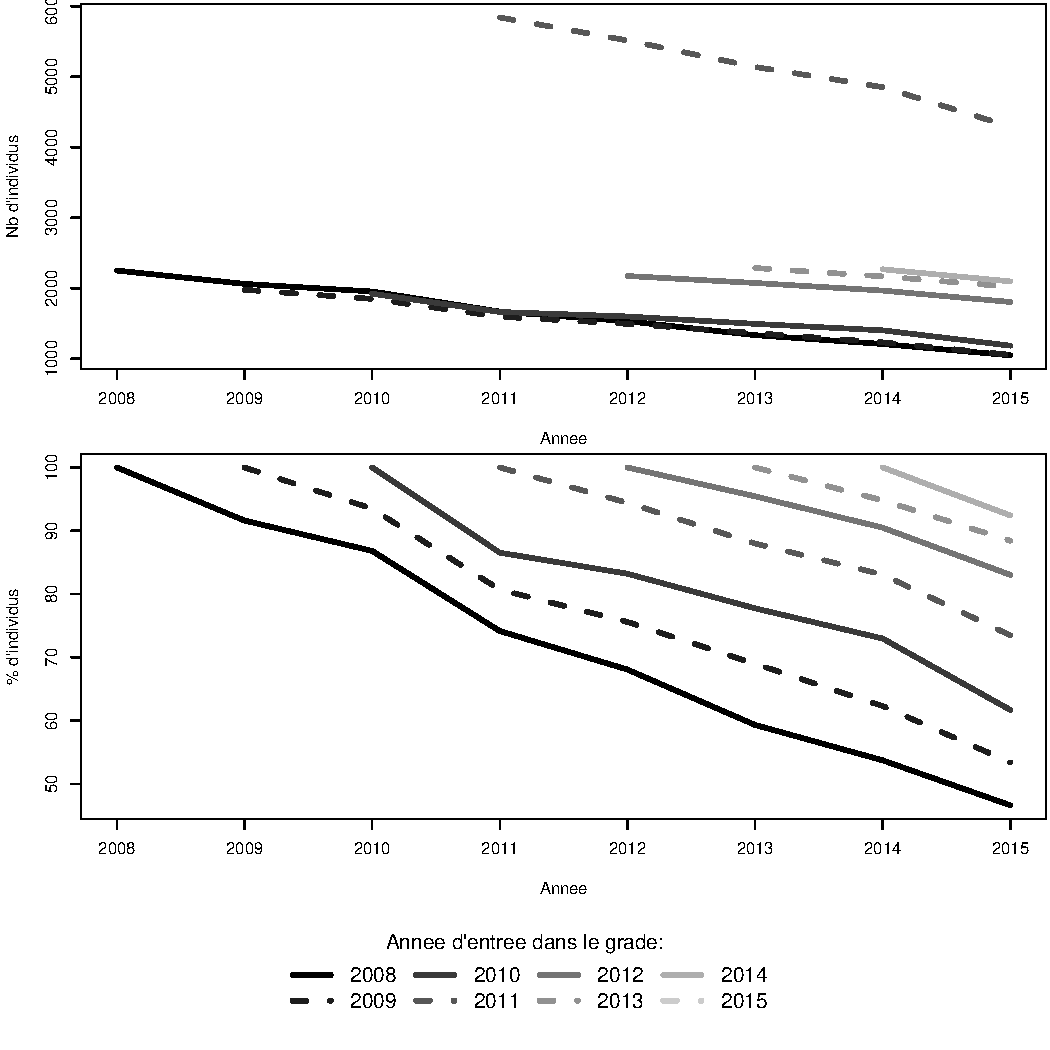
\includegraphics[width=1\linewidth]{survival_AT_1.pdf} 
    \vspace{4ex}
  \end{subfigure}
  \begin{subfigure}[b]{0.55\linewidth}
        \caption{Grade 794} 
    \label{echelon_by_neg_1} 
    \centering
    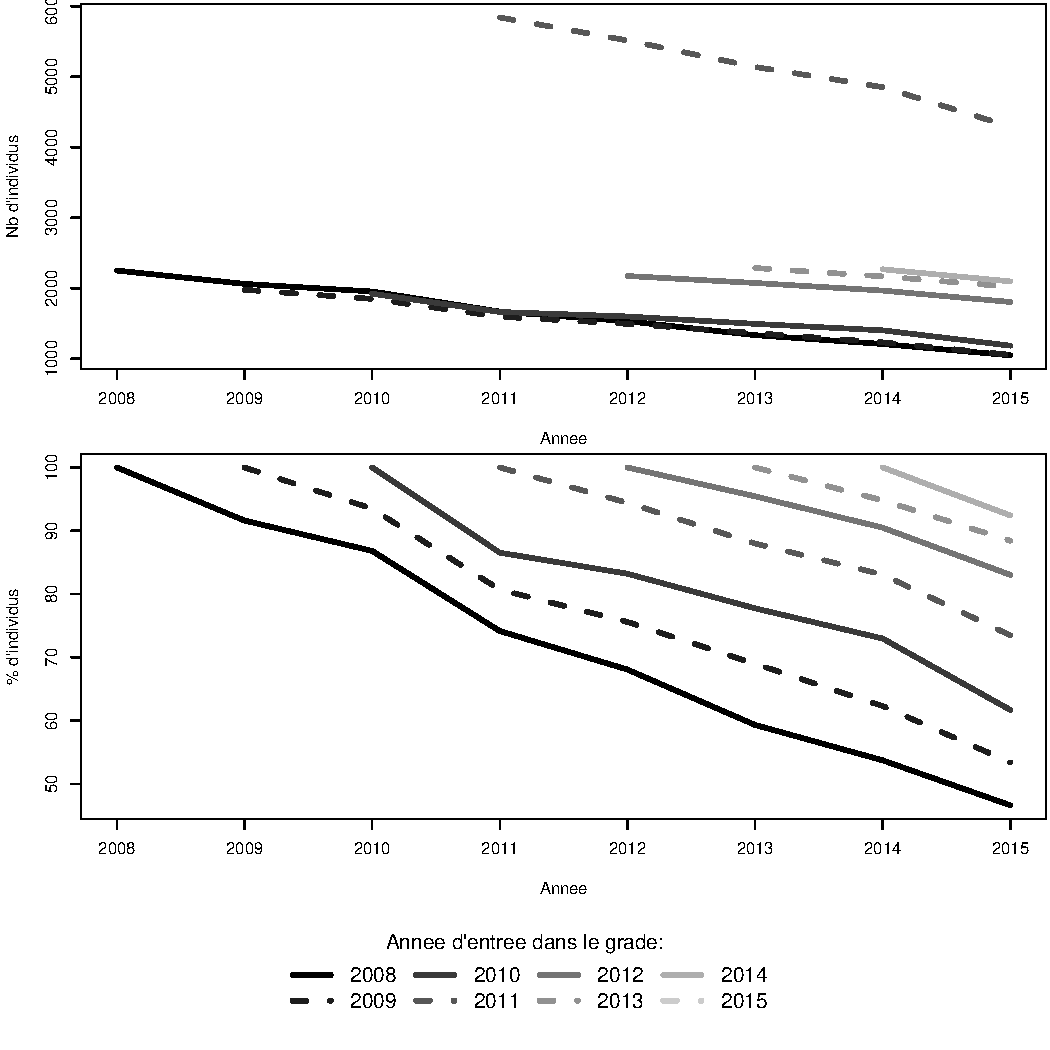
\includegraphics[width=1\linewidth]{survival_AT_2.pdf} 
    \vspace{4ex}
  \end{subfigure} 
  \begin{minipage}{12cm}
\footnotesize
\textsc{Population:} Filtres F1 et F2. Années 2007 à 2015. \\
\textsc{Lecture:} Environ 75\% des individus entrés dans le grade 793 en 2007 sont encore présents en 2011. 
\end{minipage}
\end{figure}


\begin{figure}[ht] 
  \caption{Répartitions des situations à chaque date pour les individus entrant en 2007 dans le grade 793 et encore présent dans le grade en n-1}
  \label{hazard} 
    \centering
    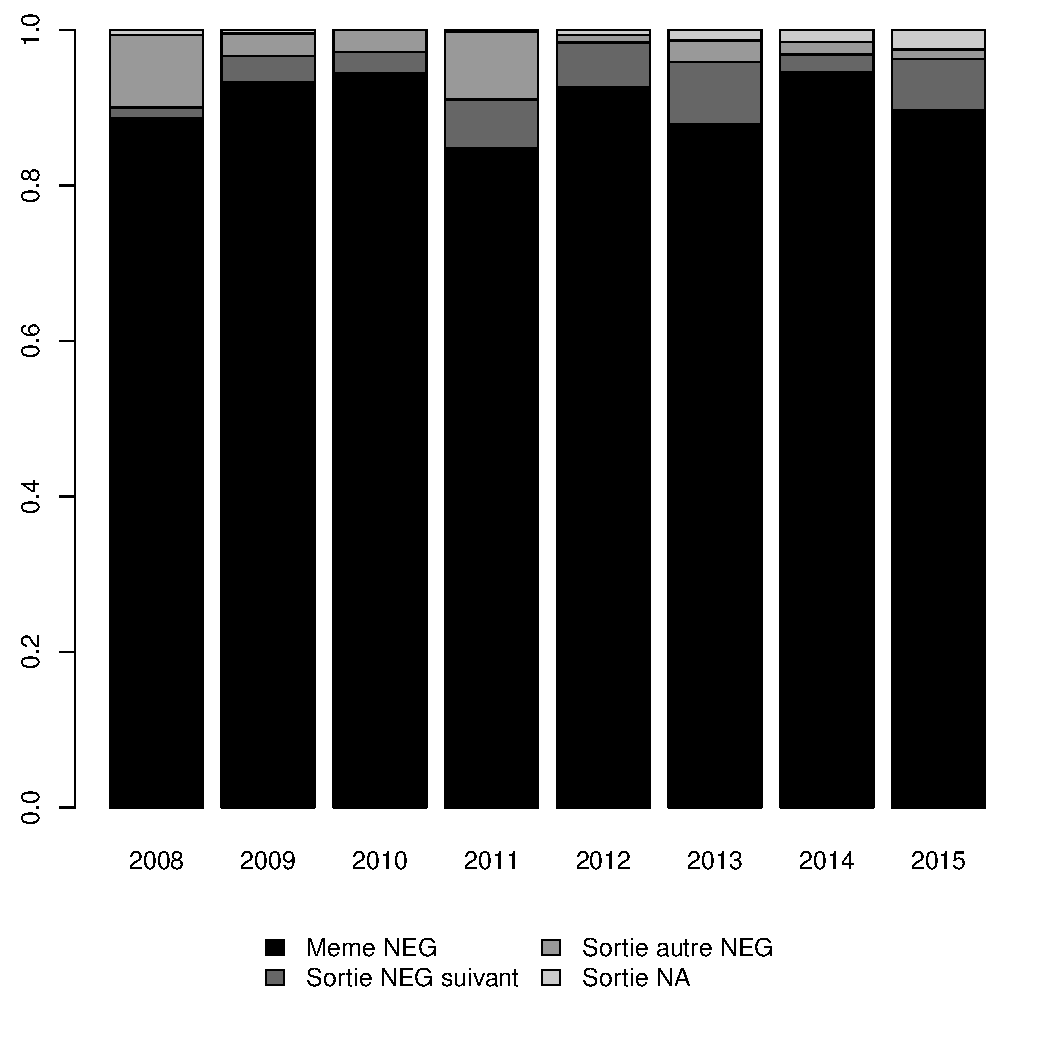
\includegraphics[width=0.75\linewidth]{destination_AT_1.pdf}  
    \begin{minipage}{12cm}
\footnotesize
\textsc{Population:} Filtres F1 et F2. Années 2007 à 2015. \\
\textsc{Lecture:} Parmi les individus entrés dans le grade 793 en 2007 et toujours dans le grade en 2010, environ 8\% part dans le grade 794, 10\% part dans un autre grade,  et le reste demeure dans le grade 793. 
\end{minipage}
\end{figure}




\clearpage
\subsection{Probabilité de sortie par échelon}

Les analyses précédentes n'intègrent pas l'échelon, car celui-ci ne semble pas correctement renseigné pour les années avant 2011.

Nous reprenons ici l'approche développée précédemment par Pierrick, en rassemblant l'ensemble des observations qu'on l'on observe pour les années les plus récentes. 

La figure \ref{evo_by_ech} présente les transitions d'une année à l'autre en fonction du grade à l'année courante (793 ou 794), vers les différents grades possibles (même grade, grade manquant, grade suivant ou autre grade) et en fonction de l'échelon à l'année courante. 

Les conditions d'éligibilité semblent bien avoir un impact, plus important encore que précédemment: c'est uniquement à partir de l'échelon d'éligibilité (4 pour le corps 793, 5 pour le corps 794) que les transitions vers le grade suivant commencent à augmenter.  

Notons toutefois les fortes transitions du grade 794 vers des grades "autres" dans les échelons inférieurs, qui constituent en réalité majoritairement des transitions vers le grade inférieur 793. Ces transitions incohérentes devront être élucidées. 

\bigskip

\begin{figure}[ht] 
  \caption{Situation d'une année à l'autre, selon l'échelon}
  \label{evo_by_ech} 
  \begin{subfigure}[b]{0.5\linewidth}
      \caption{Grade 793 à l'année courante}
    \label{evo_by_ech_0} 
    \centering
    \includegraphics[width=1\linewidth]{next_793.pdf} 
  \end{subfigure}%
  \begin{subfigure}[b]{0.5\linewidth}
        \caption{Grade 794 à l'année courante} 
    \label{evo_by_ech_1} 
    \centering
    \includegraphics[width=1\linewidth]{next_794.pdf} 
  \end{subfigure} 
\end{figure}




\clearpage
\subsection{Vitesse dans le grade et dans l'échelon}

Un dernier point devant être documenté en amont des choix de modélisation est l'importance des effets individuels dans la durée passée dans les grades ou les échelons. 

\subsubsection*{Vitesse dans le grade}

Nous laissons pour l'instant de coté cet aspect, qui nécessite un recul temporel important. 

\subsubsection*{Vitesse dans l'échelon}

Nous nous concentrons sur les années pour lesquelles l'échelon est bien renseigné (2011-2015) et adoptons la stratégie suivante: pour chaque individus de la base après application des filtres F1, F2 et F3, nous calculons la distribution de la durée passée dans le deuxième échelon observé pour les individus du grade 793 ayant au moins 2 changements d'échelons entre 2011 et 2015. Notons qu'à ce stade, à nouveau, nous considérons séparément les grades et les échelons, de sorte que nous pouvons surestimer la durée passée dans l'échelon (si l'individu change de grade mais reste dans un échelon de même niveau, nous n'identifions pas de changement d'échelon à ce stade). 

La figure \ref{duree_by_ech} présente la distribution des durées passée dans l'échelon, pour différents groupes. 
Si l'on prend l'ensemble de la population du grade (panel a), nous observons une distribution plurimodale de la durée passée dans l'échelon. Cela pourrait suggérer une forte variation interindividuelle pour ce qui est de la durée passée dans l'échelon. Mais si l'on différencie en fonction de l'échelon considérée, on constate que ces différents pics recoupent largement les différentes conditions d'avancements pour le passage à l'échelon suivants, présentées ci-dessous. 

\begin{table}[h!]
\label{means}
\centering
\caption{Conditions d'avancement pour le grade 793} 
\footnotesize
\begin{tabular}{l|cc}
\toprule
Echelon &  durée min &  durée max \\
01  &12	&12 \\
02	&24	&18 \\
03	&24	&18\\
04	&36	&24\\
05	&36	&24 \\
06	&36	&24 \\
07	&48	&36 \\
08	&48	&36 \\
09	&48	&36 \\
10	&48	&36	 \\
%	
\bottomrule
\end{tabular}
\end{table}


Ainsi par exemple nous observons une forte concentration de la durée de l'échelon à 24 mois pour les échelons 4 à 7. 
 

Certains points restent toutefois obscurs:
\begin{itemize}[leftmargin=1cm ,parsep=0cm,itemsep=0cm,topsep=0cm] 
\item Concentration à 1: souvent un changement de grade suivant un changement d'échelon?
\item Pas beaucoup de durée max, durée min = durée fixe?
\item Beaucoup de départ avant la durée min, en particulier pour les  échelons supérieurs. A nouveau, il n'est pas encore possible de savoir si cela vient d'un problème des données ou d'une application lâche des critères d'éligibilité. 
\end{itemize}



\begin{figure}[ht] 
  \caption{Durée passée dans l'échelon, en fonction de l'échelon (grade 793)}
  \label{duree_by_ech} 
    \includegraphics[scale = 0.6]{duree_ech_793.pdf} 
      \begin{minipage}{12cm}
\footnotesize
\textsc{Population:} Filtres F1, F2 et F3. Années 2011 à 2015. Individus qui ont connu au moins deux échelons entre 2011 et 2012 et qui se trouvent dans le grade 793 en 2012. 
\end{minipage}
\end{figure}






\clearpage
%\section{Premières estimations}



\clearpage
\section{Résumé et liste des points à aborder en priorité}

\subsection*{Constat d'étape et perspectives envisagées}


\begin{itemize}
\item L'approche de la modélisation de la rémunération à partir modélisation des grilles semble bien pertinente, sur la base de deux points principaux:
\begin{enumerate}
\item L'observation des trajectoires indiciaires \og en escalier \fg{} qui ne peuvent être modélisables qu'à partir des évolutions des grilles et des trajectoires des individus dans ces grilles (graphique \ref{trajectories}).
\item Quand il est possible de les identifier précisément, les conditions d'éligibilité au changement de grade semblent bien jouer un rôle important (graphique \ref{evo_by_ech}). A ce stade, il n'est pas possible de vérifier l'impact joint des deux types de conditions (échelon, durée dans le grade), car la condition de durée de grade nécessite un recul temporel important et que les échelons ne sont bien renseignés que pour les années récentes. 
\end{enumerate}
\item Toutefois, la possibilité de mise en oeuvre de l'approche n'est pas encore assurée, du fait des doutes persistants sur la qualité des données, malgré un investissement déjà lourd. A ce stade, même sur un échantillon restreint \textit{a priori} favorable, nous ne sommes pas en mesure de reconstituer de manière fiable les trajectoires (grade, échelon) avec une profondeur minimale (2007-2015). 

\item Nous proposons donc les perspectives de travail suivantes:
\begin{enumerate}
\item Poursuivre la mise en oeuvre de l'approche par grille, en visant à l'amélioration de données, en particulier avant 2011. Dans un premier temps nous pourrions nous concentrer sur quelques corps de la fonction publique territoriale pour lesquels nous viserions un taux de remplissage de l'ordre de 80\% et une reconstitution de l'historique des conditions d'avancement. 
\item Mettre en oeuvre de manière assez rapide une méthodologie alternative sur la base d'équations de salaire classique, idéalement sur la base de ce qu'a mis en place le SRE. Cette option comporte deux avantages notables:
\begin{enumerate}
\item L'apport de l'approche par grille ne pourra etre évaluée que sur la base de ce qui se fait habituellement pour la modélisation des rémunérations. Cela justifie en soi l'estimation d'équation de salaire à des fins de comparaison. 
\item En outre, cela limiterait le risque à court terme en ne conditionnant pas la mise en oeuvre de l'ensemble du modèle à la modélisation des trajectoires dans les grilles. 
\end{enumerate} 
\end{enumerate}

\end{itemize}


\subsection*{Autres points à discuter}


\begin{enumerate}

\item Information sur les grilles: 
\begin{itemize}[leftmargin=1cm ,parsep=0cm,itemsep=0cm,topsep=0cm] 
\item Historique des conditions d'avancement
\item En pratique, quelle degré de contrainte pour les grilles (condition d'avancement pour grade et échelon) ? 
\end{itemize}

\item Amélioration des données 
\begin{itemize}[leftmargin=1cm ,parsep=0cm,itemsep=0cm,topsep=0cm] 
\item Améliorer le remplissage des neg 
	\begin{enumerate}[leftmargin=1cm ,parsep=0cm,itemsep=0cm,topsep=0cm] 
	\item Poursuivre le matching
	\item Renseigner des grades à la main 
	\item Matching sur une sous-population de libellés des individus ayant au moins un NEG dans le corps
	\end{enumerate}
\item Correction du grade à partir de l'indice. 
\item Prolongation de l'étape 1 en rétrospectif?
\end{itemize}

\item Modélisation
\begin{itemize}
\item Logit vs. modèles de durée
\item Arbitrage validité interne vs. externe
\end{itemize}



\end{enumerate}




%
%\section*{Annexes}
%
%\subsection{Résultats pour les adjoints administratifs}
%
%\begin{figure}[ht] 
%  \caption{Survie dans le grade: Adjoints administratifs}
%  \label{echelon_by_neg} 
%  \begin{subfigure}[b]{0.55\linewidth}
%      \caption{Grade AA2} 
%    \label{echelon_by_neg_0} 
%    \centering
%    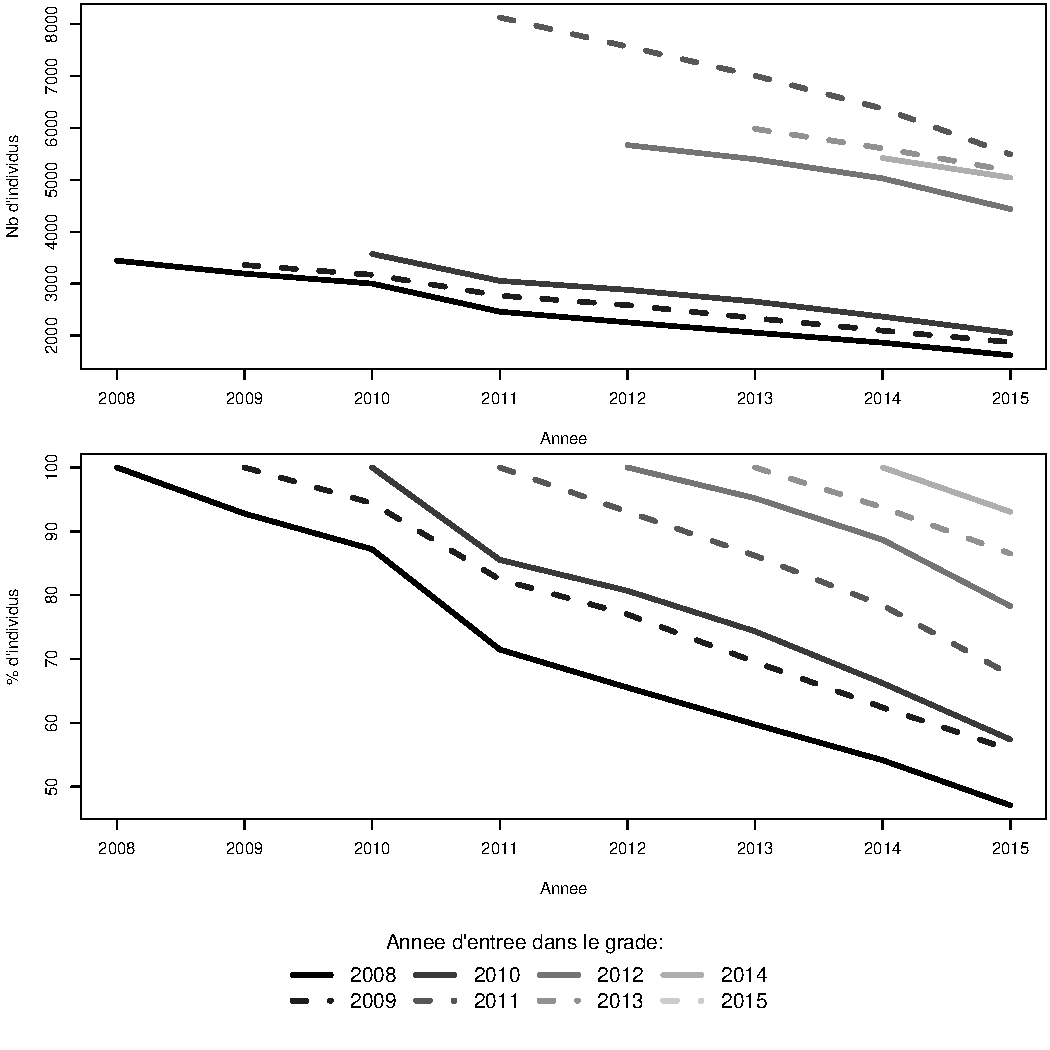
\includegraphics[width=1\linewidth]{survival_AA_1.pdf} 
%    \vspace{4ex}
%  \end{subfigure}
%  \begin{subfigure}[b]{0.55\linewidth}
%        \caption{Grade AA1} 
%    \label{echelon_by_neg_1} 
%    \centering
%    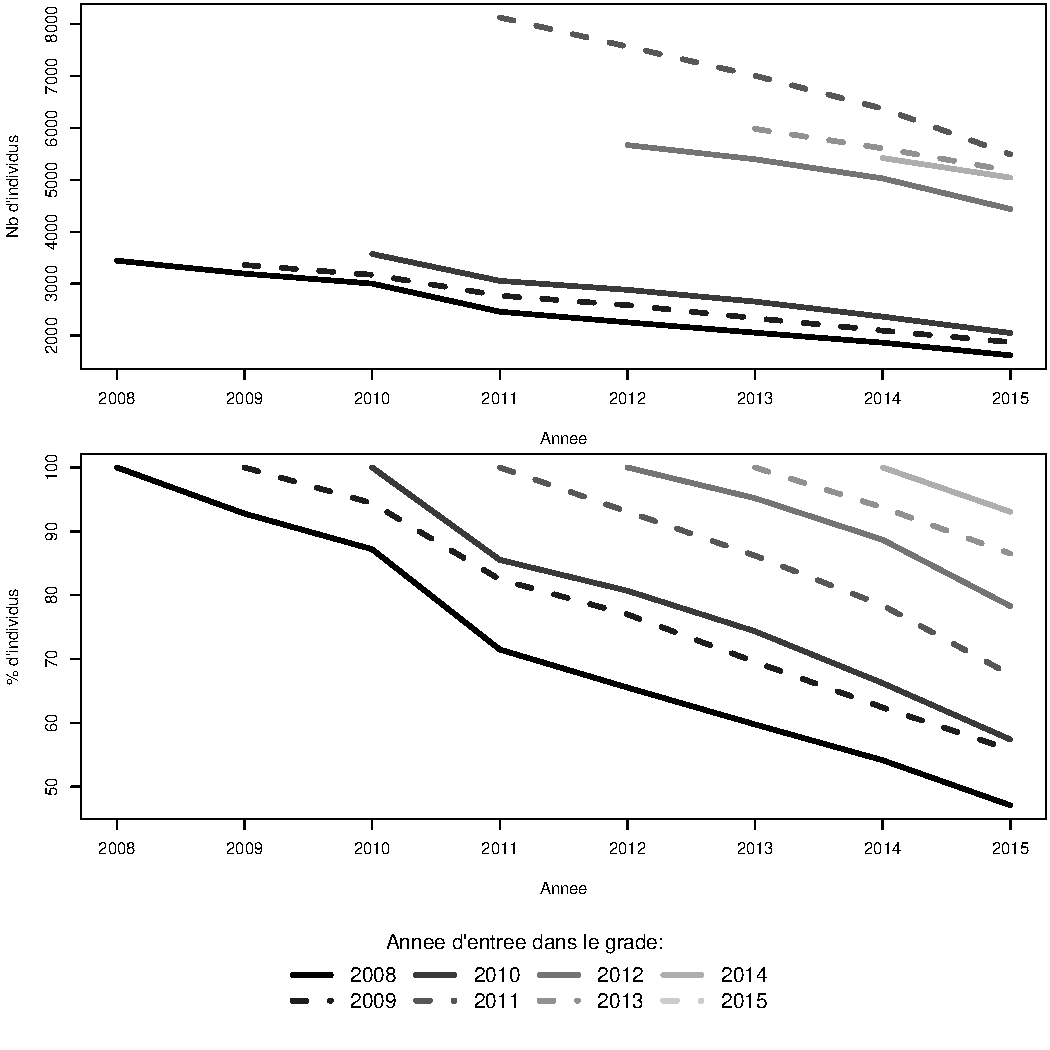
\includegraphics[width=1\linewidth]{survival_AA_2.pdf} 
%    \vspace{4ex}
%  \end{subfigure} 
%  \begin{minipage}{12cm}
%\footnotesize
%\textsc{Population:} Filtres F1 et F2. Années 2007 à 2015.
%\textsc{Lecture:} .
%\end{minipage}
%\end{figure}
%
%
%\subsection{Résultats pour les aides soignants}




\end{document}


